\documentclass[16pt, aspectratio=43,compress]{beamer}

% Add paths to look through
\makeatletter
\def\input@path{{Classes/}{preface/}{introduction/}{method/}{structure/}{dynamics/}{crystallisation/}{conclusion/}{appendix/}}
\makeatother

\mode<presentation>
{
  \usetheme{Ilmenau}
  \useoutertheme{myframes}
}

\usepackage{common}
\usepackage{tikz}
\usepackage{textpos}
\usepackage{multimedia}
\usepackage{media9}
\usepackage{pgfpages}
\usepackage[cm]{sfmath}
\usepackage{animate}

\usepackage[backend=biber]{biblatex}
\addbibresource{bibliography/crystal.bib}

\graphicspath{{preface/figures/}{method/figures/}{introduction/figures/}{dynamics/figures/}{structure/figures/}{crystallisation/figures/}{presentation/}}
\renewcommand{\footcite}{\footfullcite}

\DeclareCiteCommand{\onlinecite}%[\mkbibbrackets]
    {\usebibmacro{cite:init}%
    \usebibmacro{prenote}}
    {\usebibmacro{citeindex}%
    \usebibmacro{cite:comp}}
    {}
    {\usebibmacro{cite:dump}%
    \usebibmacro{postnote}}

\setbeamertemplate{navigation symbols}{}

\renewcommand{\footnoterule}{}
%\renewcommand{\footnotemark}{}
\renewcommand*{\footnotesize}{\fontsize{5}{7}}

\makeatletter
\def\@listi{\leftmargin\leftmargini
              \topsep    2ex
              \parsep    0\p@   \@plus\p@
              \itemsep   4ex}
\makeatother

\newcommand*{\myhat}[1]{\skew{3}{\hat}{#1}}

%\title[Shapes on a Plane]{The Role of Molecular Shape on the Properties of the Condensed Phase:\\ A Simulation Study}
\author{Malcolm Ramsay}
\title[Shapes on a Plane]{}

\usecolortheme{whale}
\usefonttheme{professionalfonts}

%\setbeameroption{show notes on second screen}

\setbeamerfont{frametitle}{size={\fontsize{22}{24}}}

\begin{document}

%%%%%%%%%%%%%%%%%%%%%%%%%%%%%%%%%%%%%%%%%%%%%%%%

\begin{frame}
    \centering
    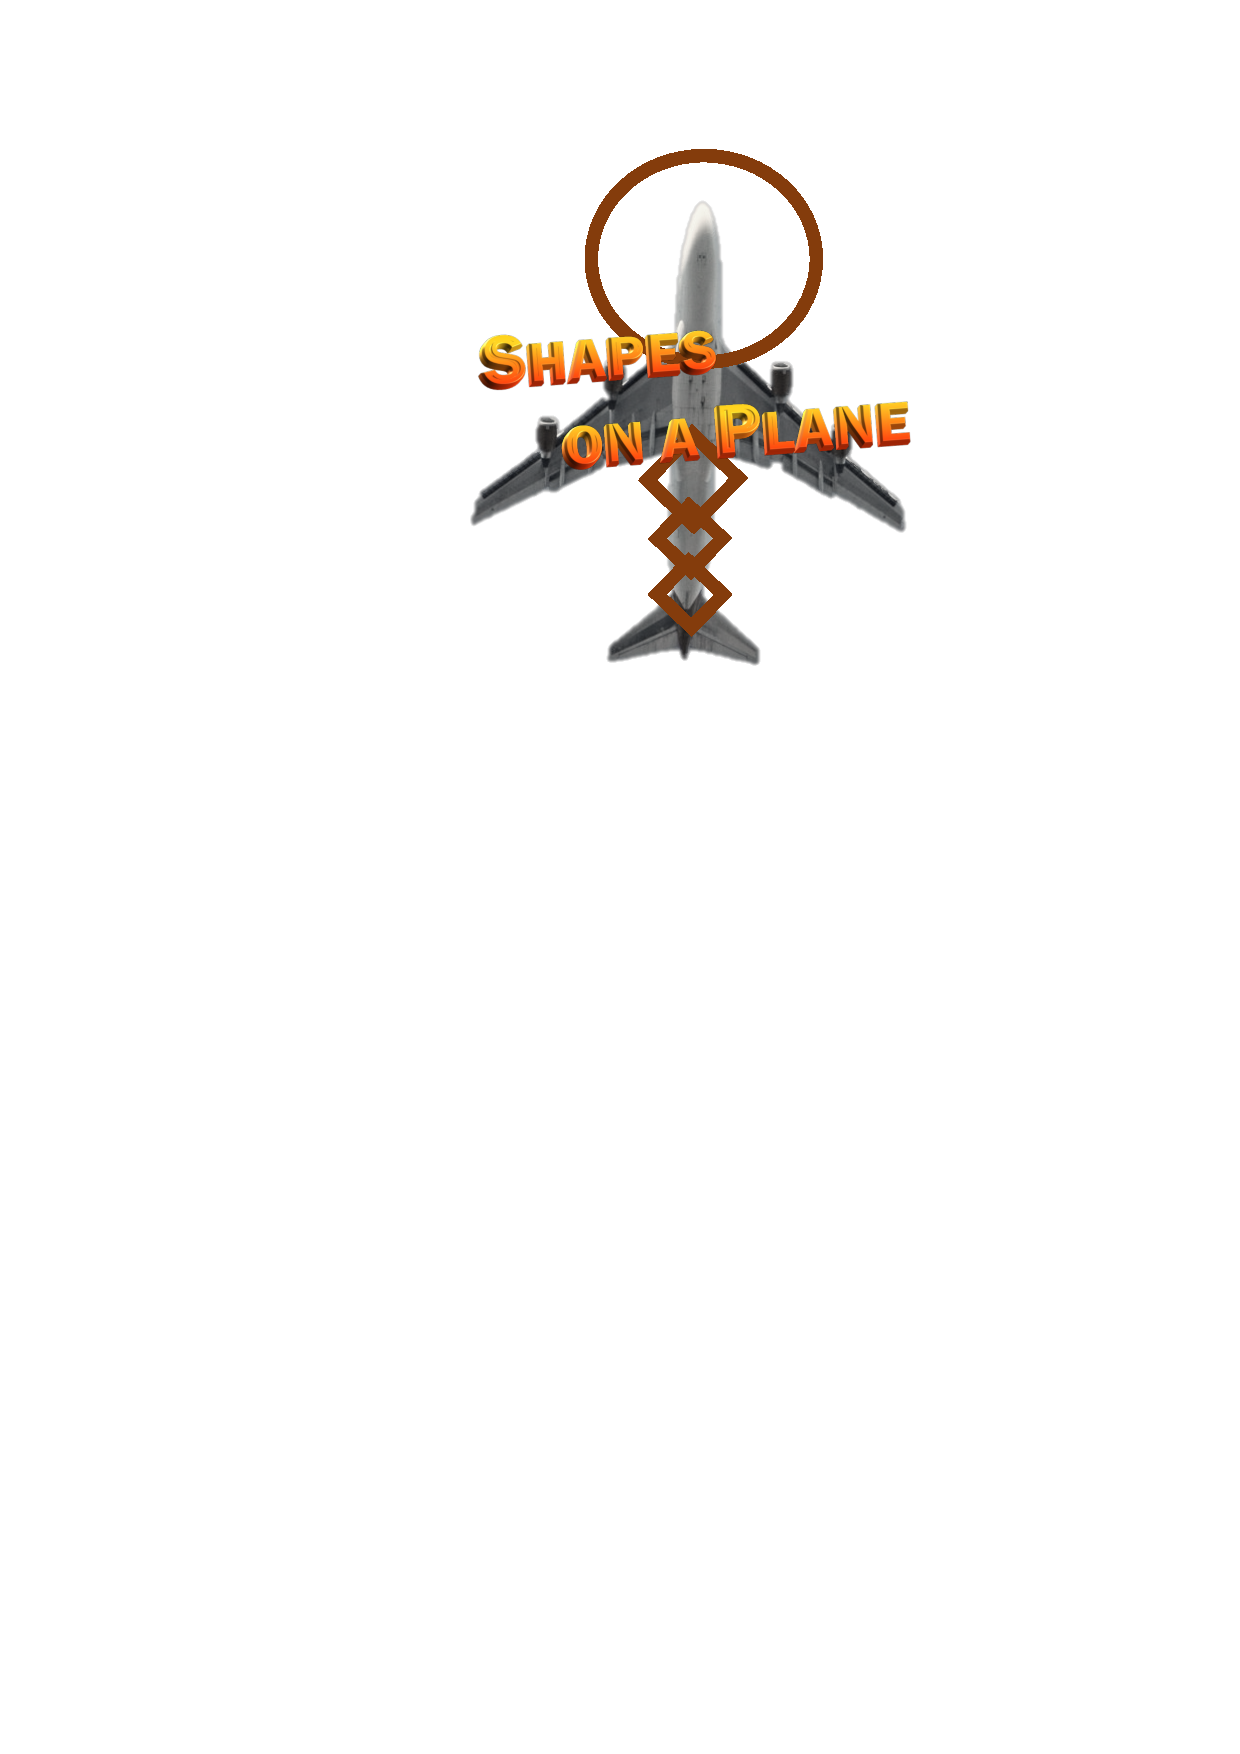
\includegraphics[height=\textheight]{shapes-plane}
    %\titlepage
\end{frame}


%%%%%%%%%%%%%%%%%%%%%%%%%%%%%%%%%%%%%%%%%%%%%%%

\begin{frame}{Outline}
    \tableofcontents
\end{frame}

\section{Introduction}
\stepcounter{subsection}

\begin{frame}{Supercooled Liquids}
    \begin{columns}
        \begin{column}{0.5\linewidth}
            \begin{itemize}
                \item Liquid below the freezing point
                \item An integral part of crystallisation
                \item Temperatures at which nucleation becomes stable
            \end{itemize}
        \end{column}
        \begin{column}{0.5\linewidth}
            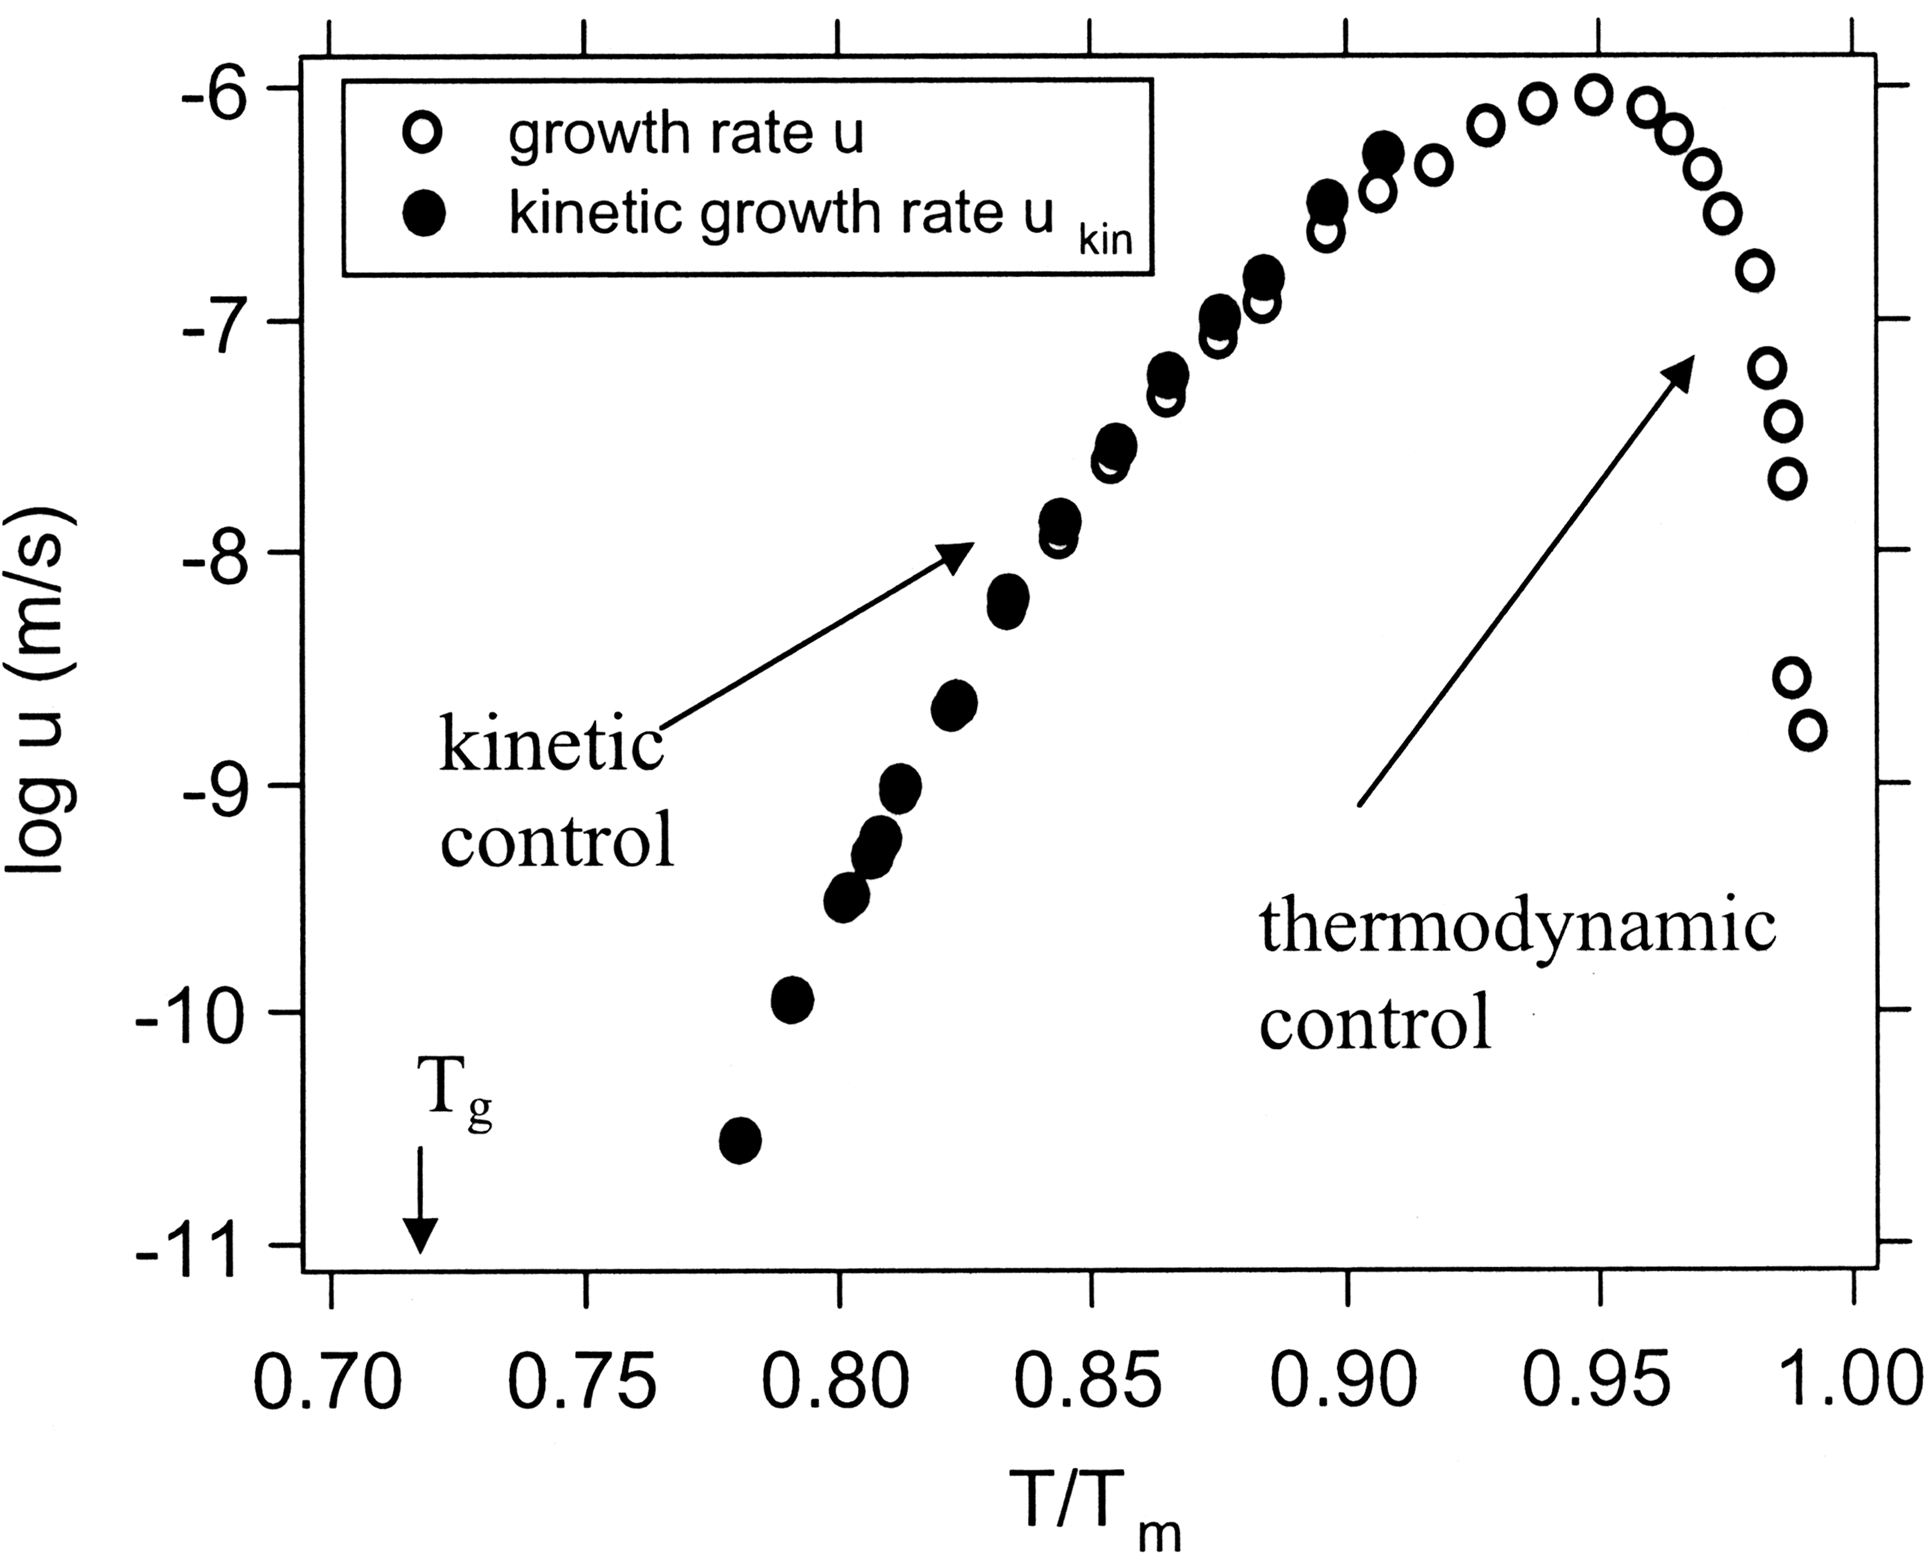
\includegraphics[width=\textwidth]{crystal-growth}
        \end{column}
    \end{columns}
\end{frame}

\begin{frame}{Liquid Fragility}
    \begin{columns}
        \begin{column}{0.5\linewidth}
            \begin{itemize}
                \item Description of liquid behaviour close to glass transition
                \item Silica (\ce{SiO2}) a strong liquid shows linear behaviour
                \item {\em o}-Terphenyl a weak liquid large deviation from linear
            \end{itemize}
        \end{column}
        \begin{column}{0.5\linewidth}
            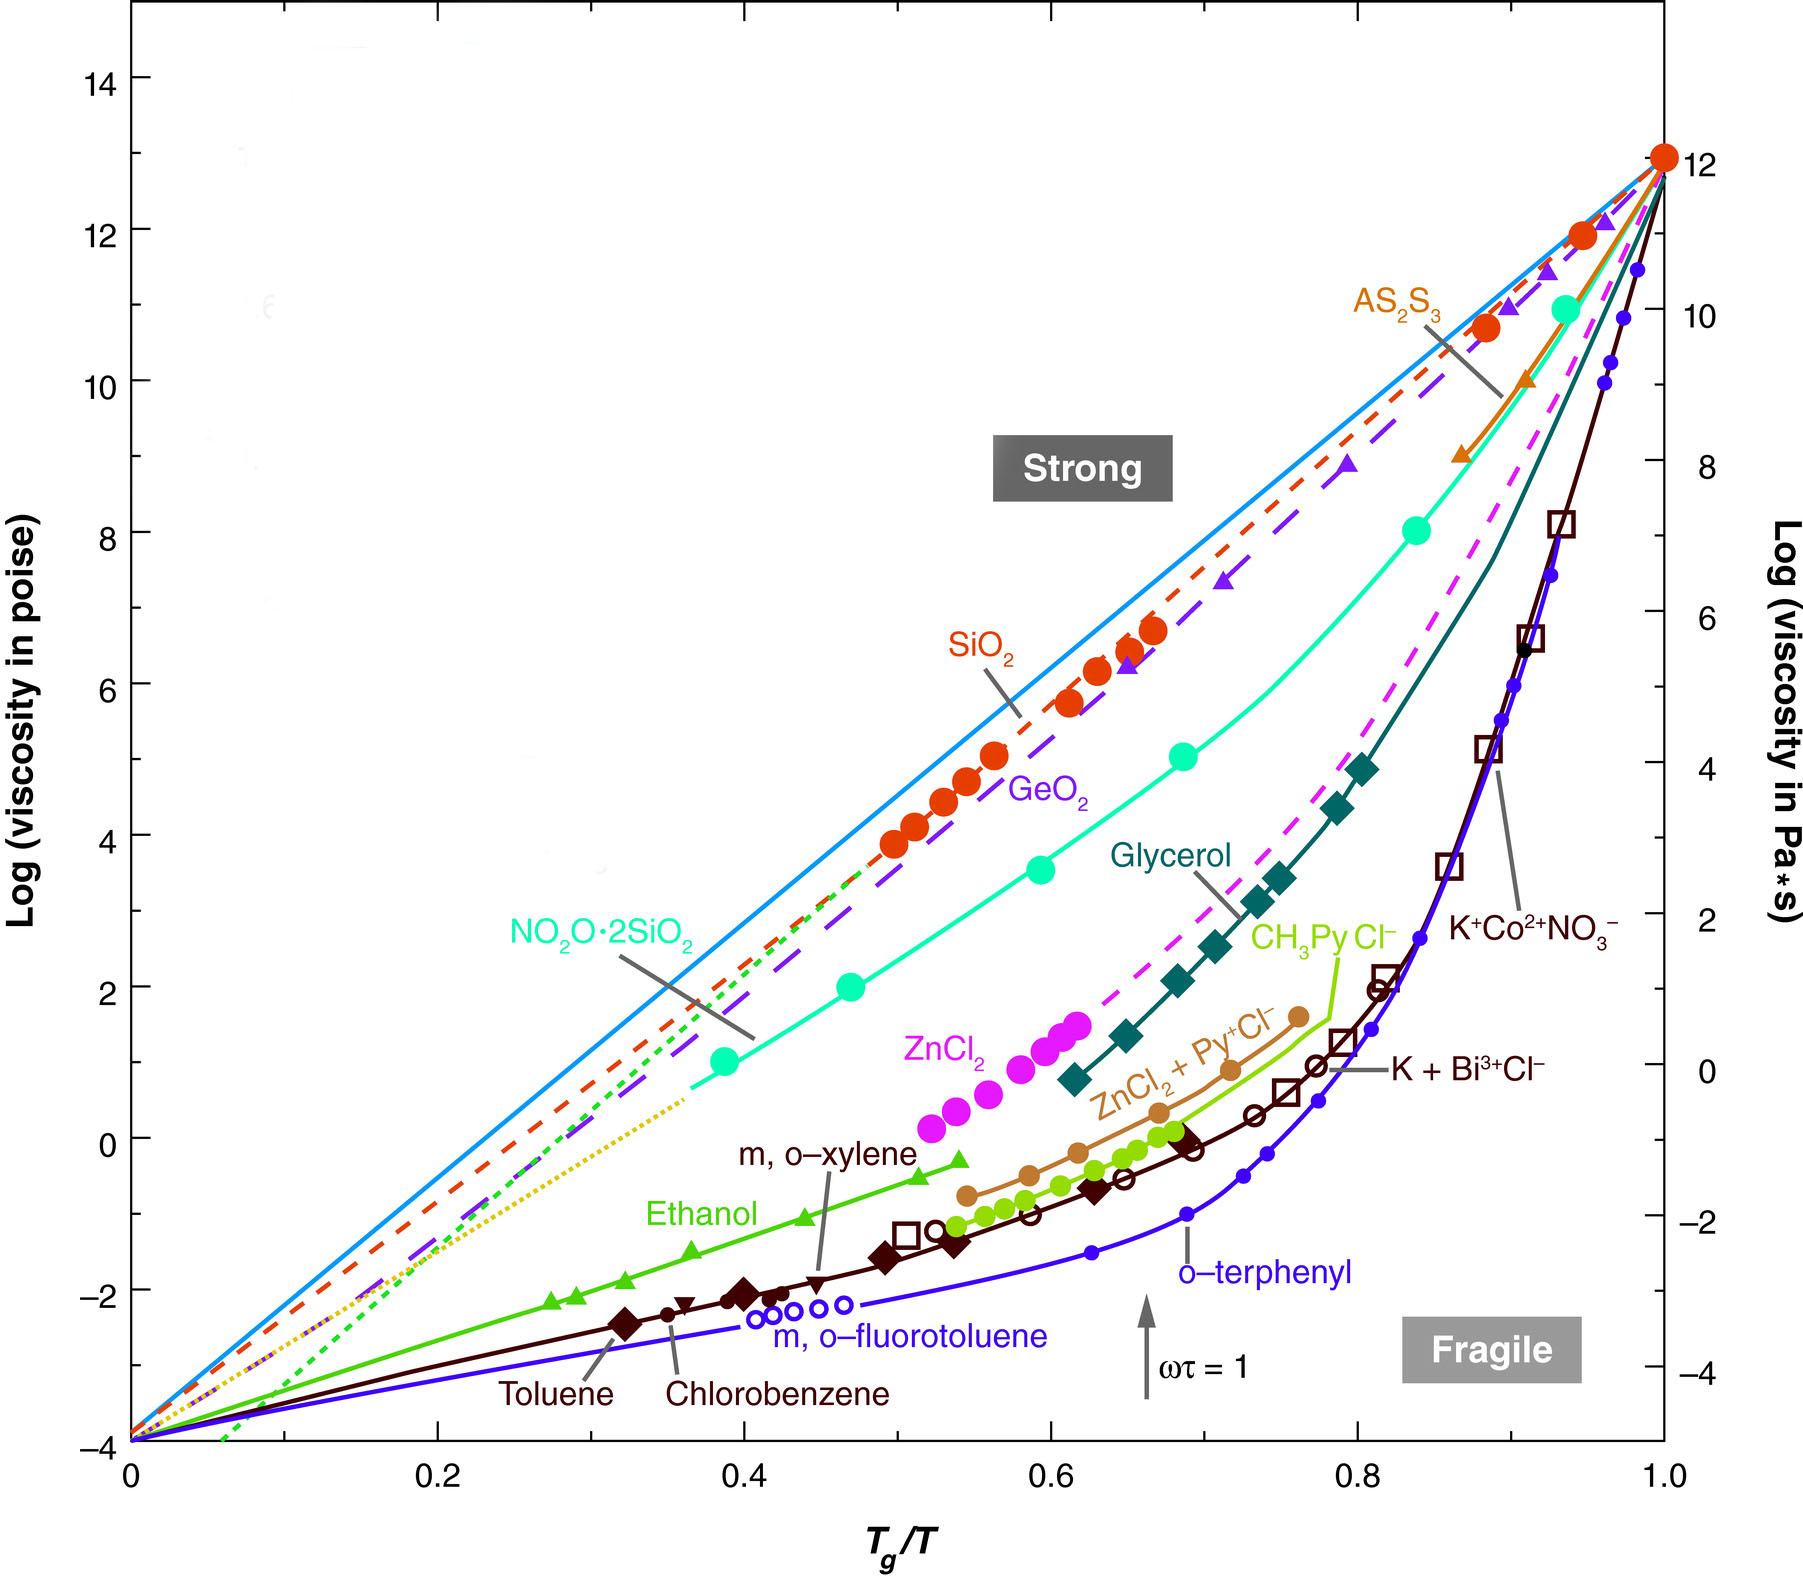
\includegraphics[width=\textwidth]{angell}
        \end{column}
    \end{columns}
\end{frame}


\section{Molecules}
\stepcounter{subsection}

\begin{frame}{Molecules Chosen for Study}
    \begin{columns}
        \begin{column}{0.3\linewidth}
            \centering
            \includegraphics[width=\textwidth]{sone}\\
            \done
        \end{column}
        \begin{column}{0.3\linewidth}
            \centering
            \includegraphics[width=\textwidth]{scon}\\
            \dcon
        \end{column}
        \begin{column}{0.3\linewidth}
            \centering
            \includegraphics[width=\textwidth]{tri}\\
            \tri
        \end{column}
    \end{columns}
\end{frame}

\section{Dynamics}
\stepcounter{subsection}

\begin{frame}{Mean Squared Displacement}
    \begin{columns}
        \begin{column}{0.5\linewidth}
            \begin{itemize}
                \item Measure of the motion of the centers of mass
            \end{itemize}
            \begin{align*}
                MSD(t) &= \langle \delta(t)^2 \rangle,\\
                \delta(t) &= \sqrt{(x(t) - x_0)^2 + (y(t) - y_0)^2}
            \end{align*}
            \begin{itemize}
                \item Summarised by the diffusion constant $D$
            \end{itemize}
            \begin{align*}
                D = \ddiff{MSD}{t}
            \end{align*}
        \end{column}
        \begin{column}{0.5\linewidth}
            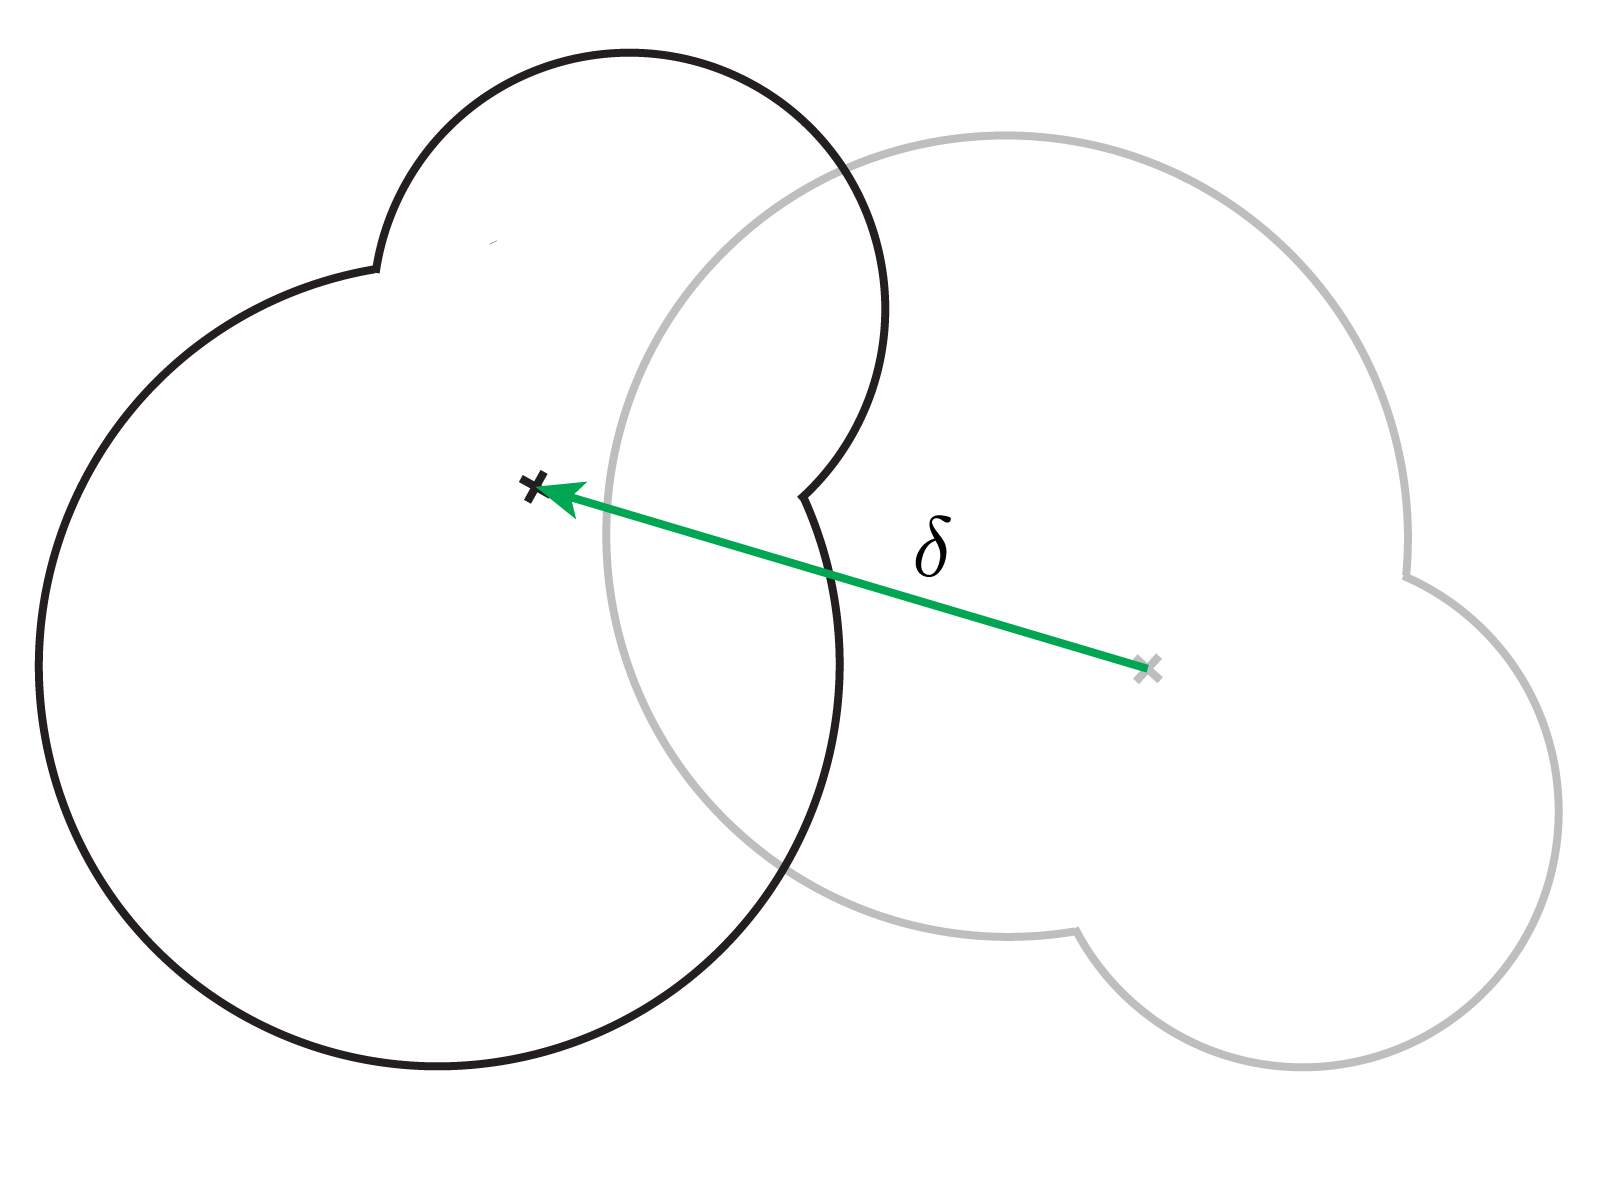
\includegraphics[width=\textwidth]{msd}
        \end{column}
    \end{columns}
\end{frame}

\begin{frame}{Diffusion Constant}
    \centering
    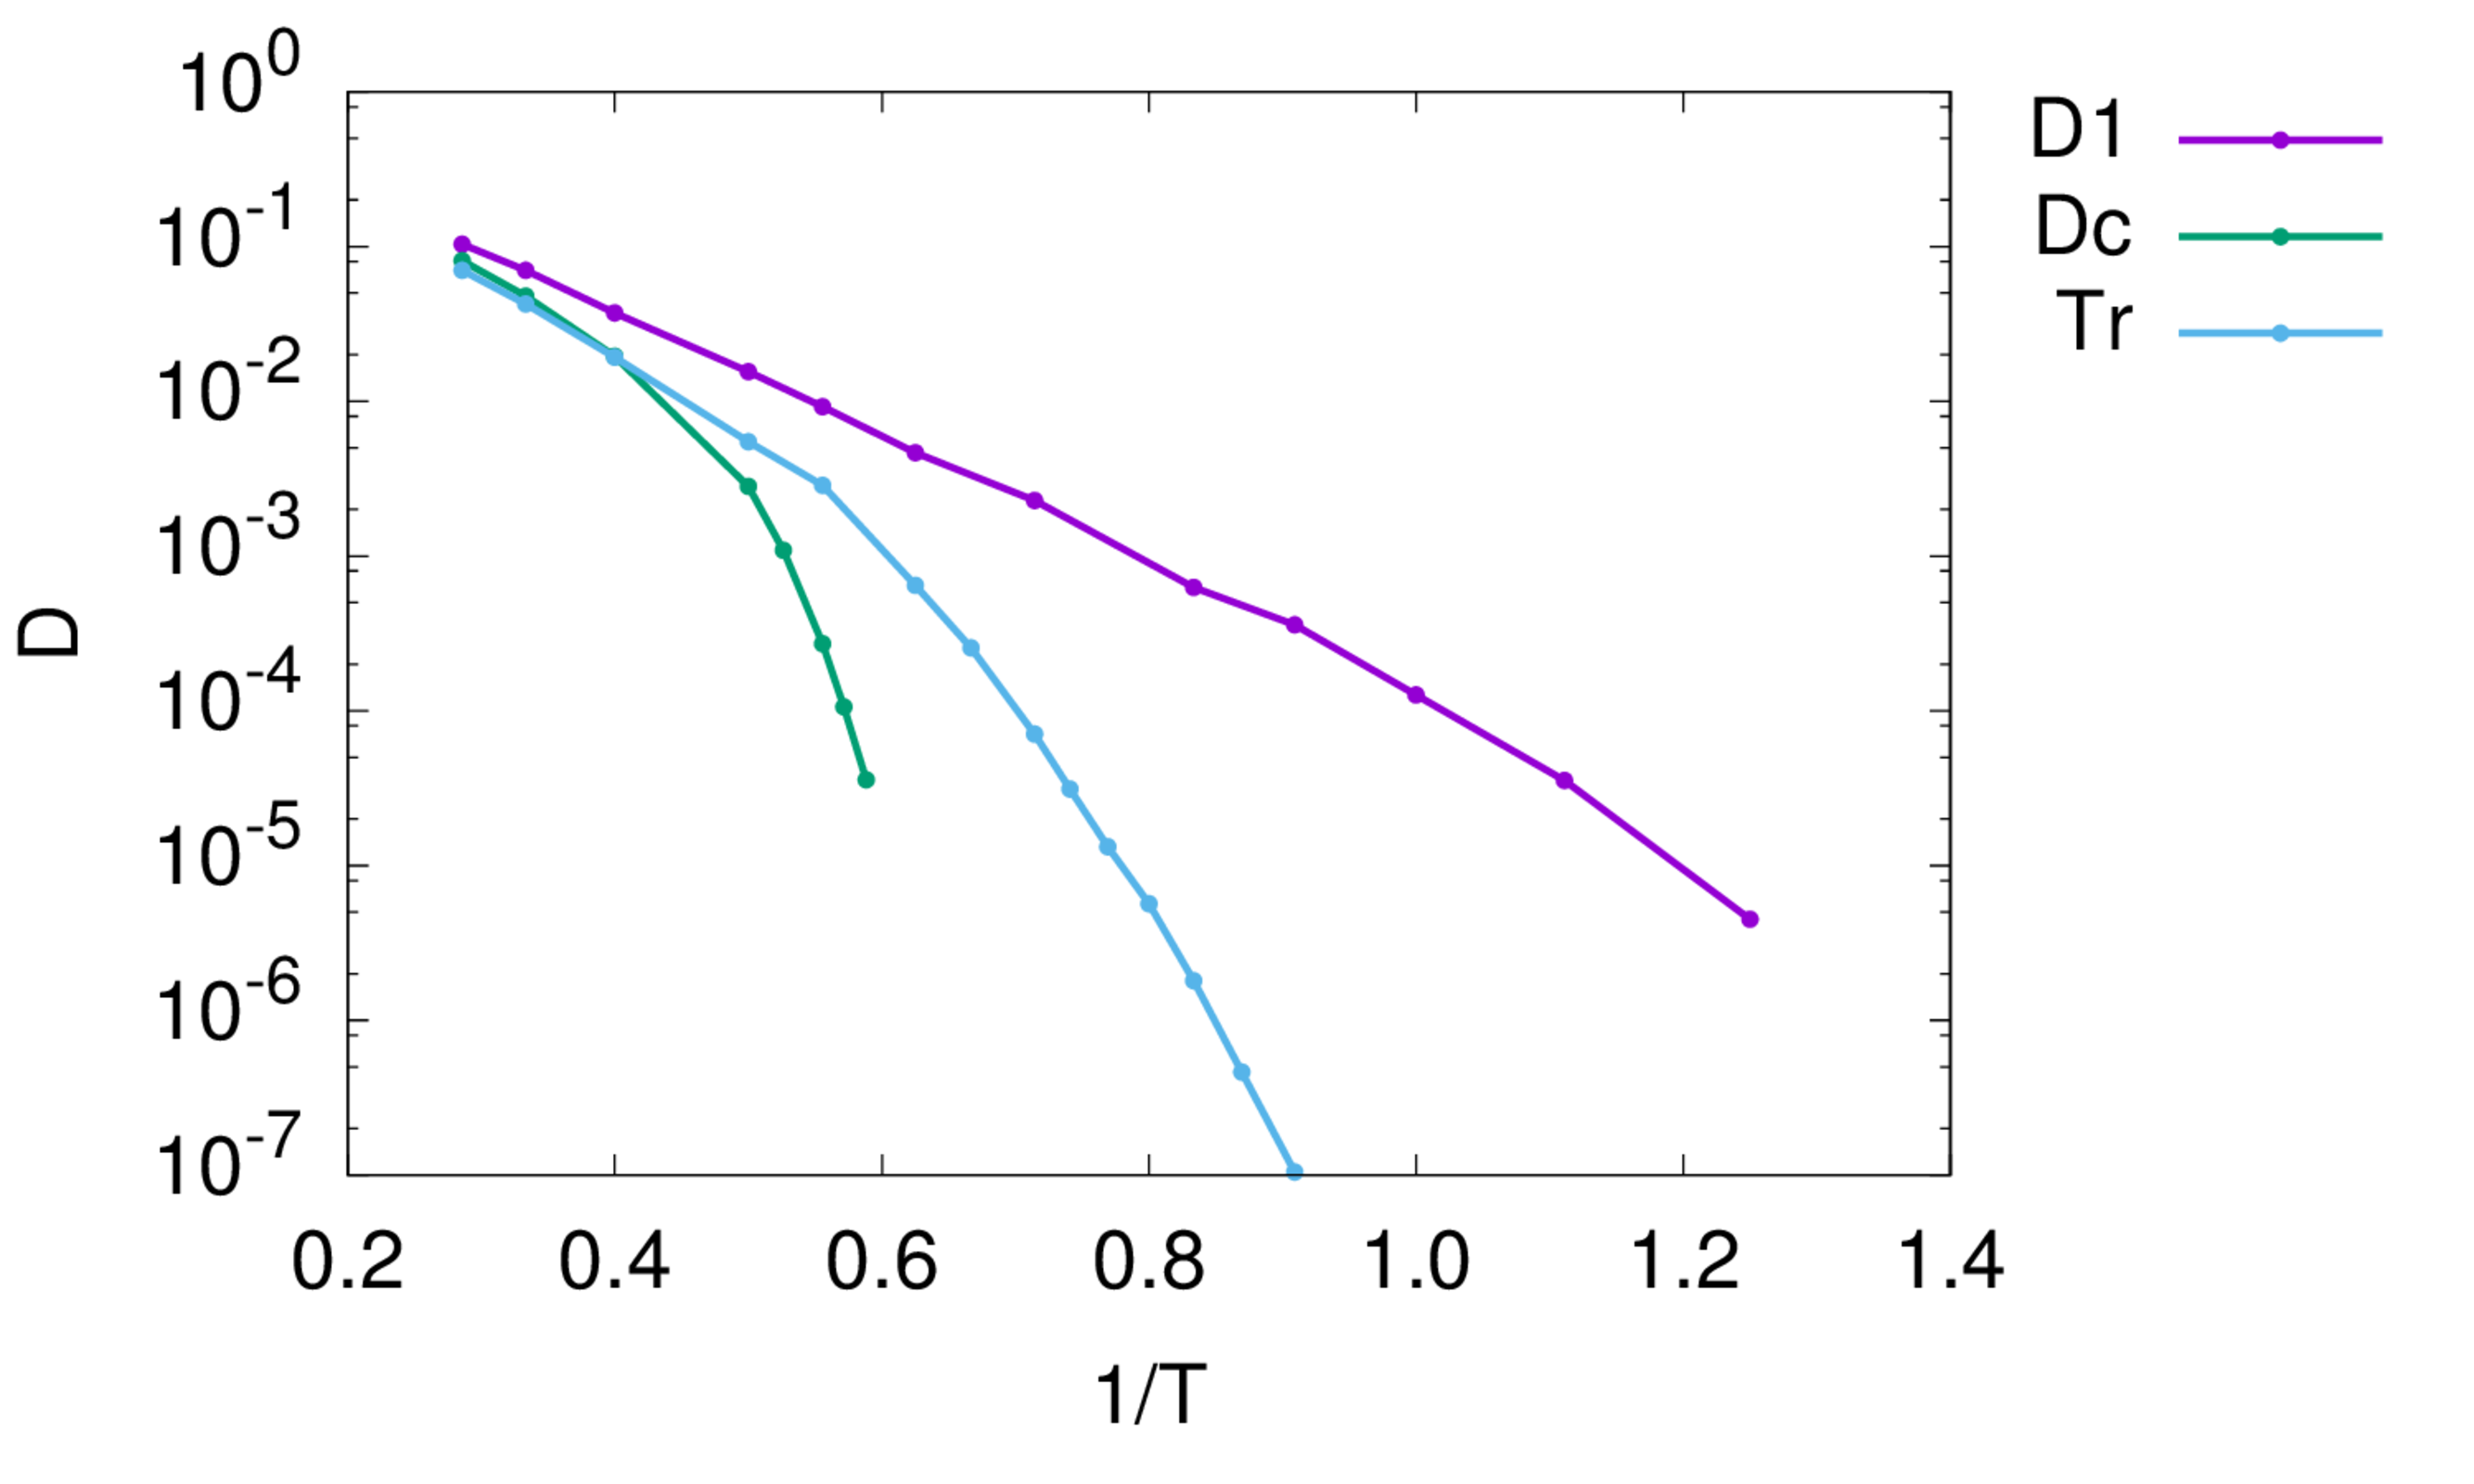
\includegraphics[width=\textwidth]{D}
\end{frame}

\begin{frame}{Rotational Relaxation}
    \begin{columns}
        \begin{column}{0.5\linewidth}
            \begin{itemize}
                \item Measure of the rotational motion
            \end{itemize}
            \begin{align*}
                C_1(t) &= \langle \vect{\hat e}(0) \cdot \vect{\hat e}(t) \rangle
            \end{align*}
            \begin{itemize}
                \item Summarised as time to reach $1/\e$
            \end{itemize}
        \end{column}
        \begin{column}{0.5\linewidth}
            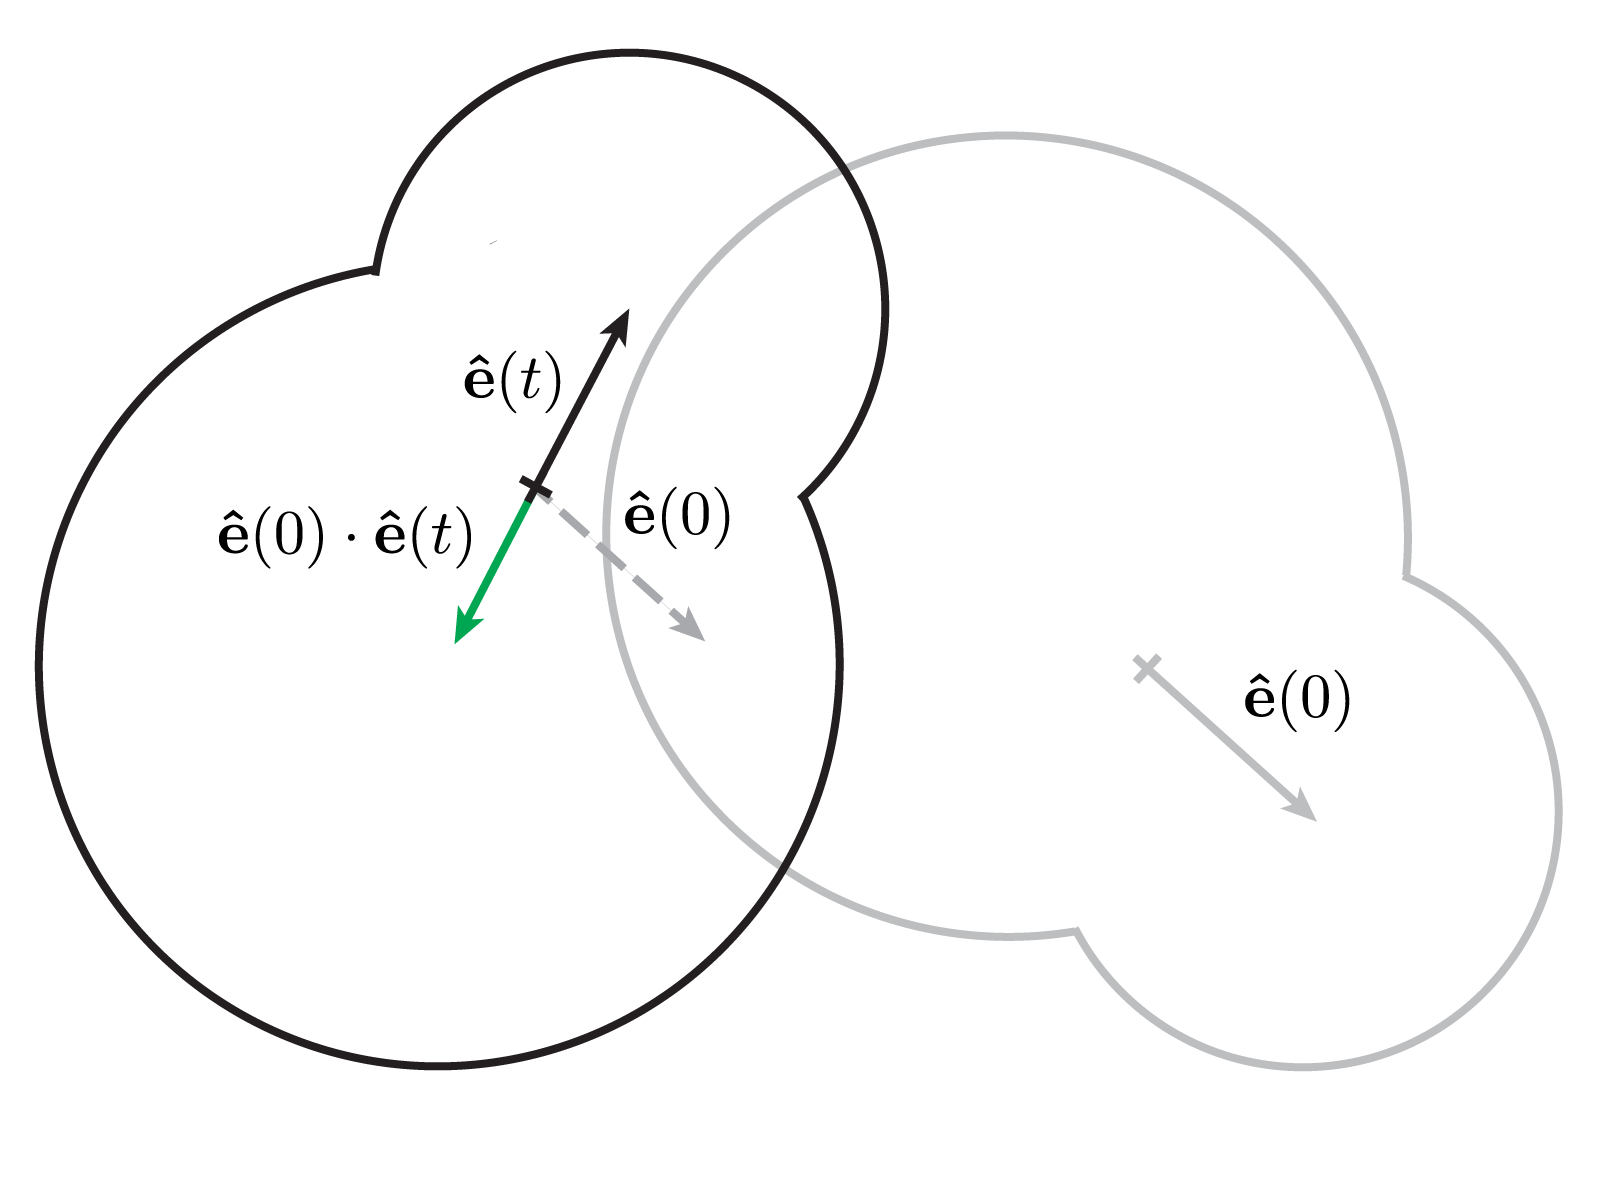
\includegraphics[width=\textwidth]{rot}
        \end{column}
    \end{columns}
\end{frame}

\begin{frame}{Rotational Relaxation}
    \centering
    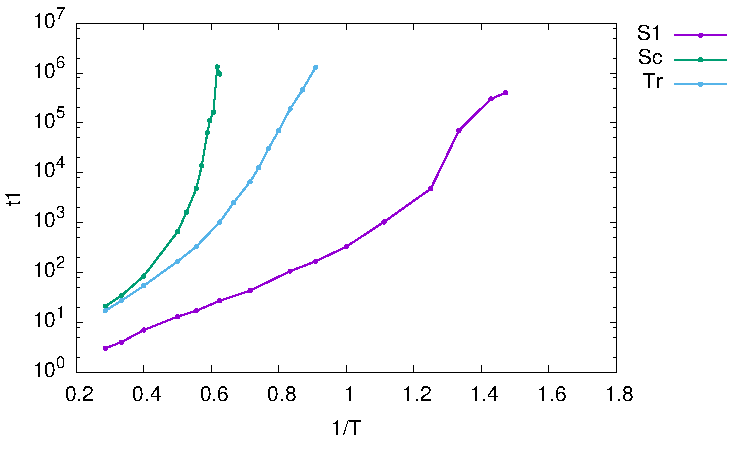
\includegraphics[width=\textwidth]{t1}
\end{frame}

\begin{frame}{Structural Relaxation}
    \begin{columns}
        \begin{column}{0.5\linewidth}
            \begin{itemize}
                \item Measure of the relaxation of the structure
            \end{itemize}
            \begin{align*}
                F(t) = \left \langle \begin{cases}
                    \quad0 &\text{if}\quad \delta  > 0.3 \\
                    \quad1 &\text{if}\quad \delta \leq 0.3
                \end{cases} \quad \right \rangle
            \end{align*}
            \begin{itemize}
                \item Summarised as time to reach $1/\e$
            \end{itemize}
        \end{column}
        \begin{column}{0.5\linewidth}
            \centering
            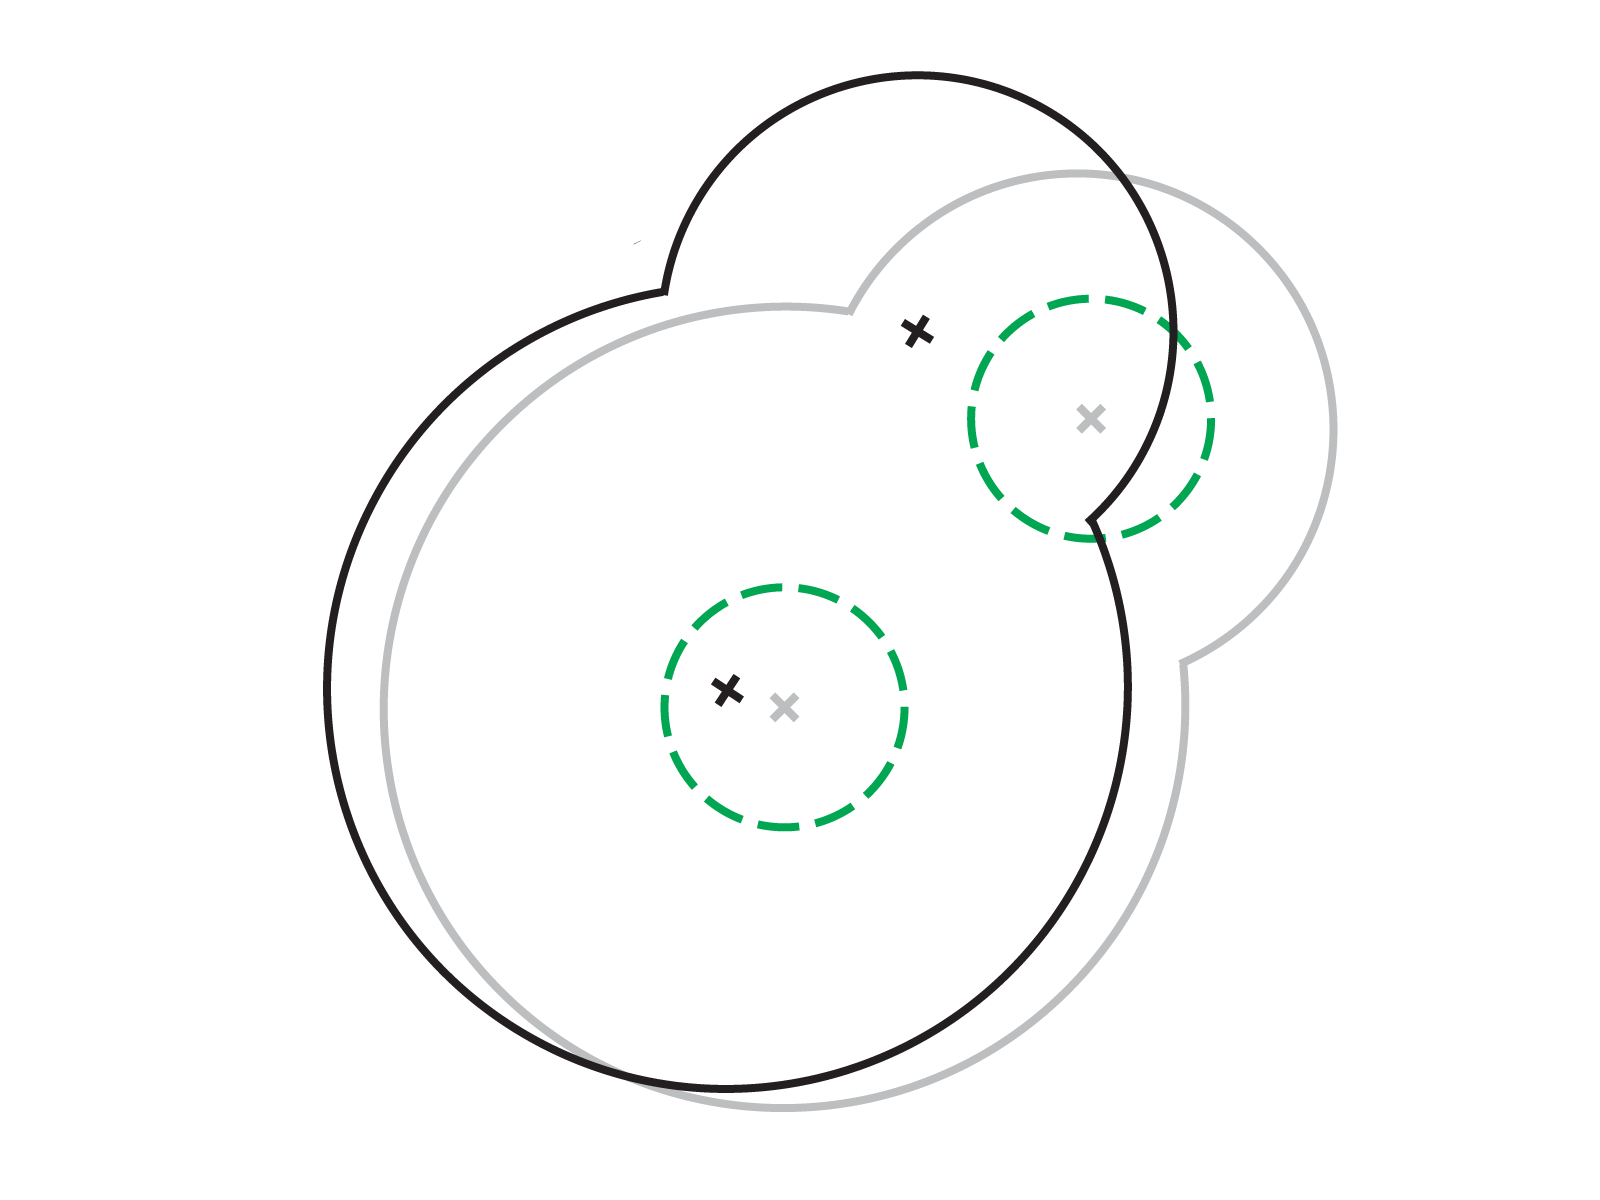
\includegraphics[width=\textwidth]{struct}
        \end{column}
    \end{columns}
\end{frame}

\begin{frame}{Structural Relaxation}
    \centering
    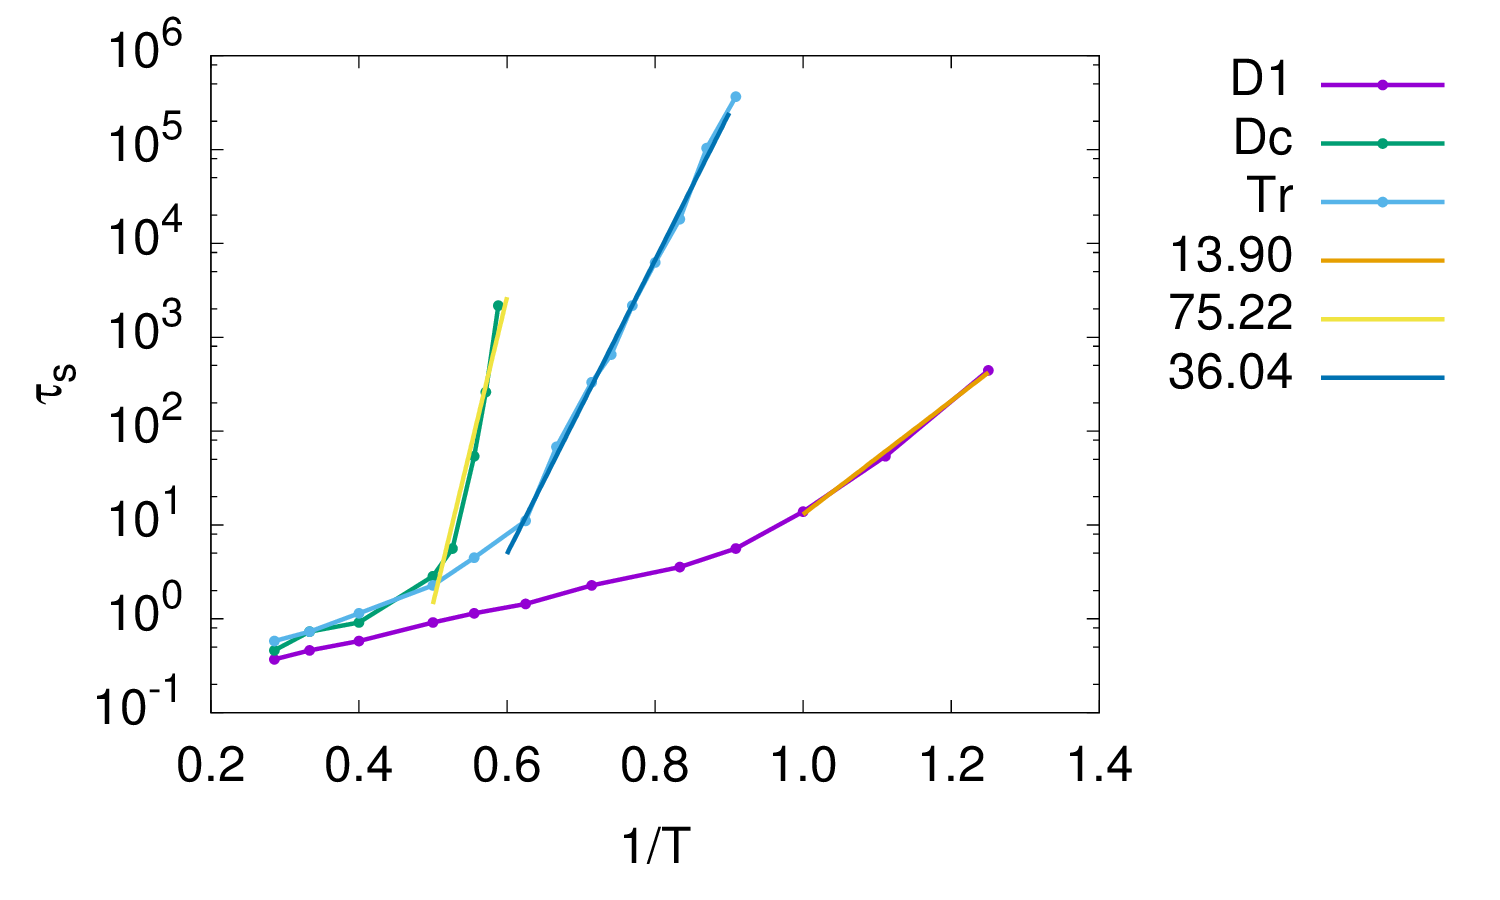
\includegraphics[width=\textwidth]{ts}
\end{frame}

\begin{frame}{Debye-Waller Factor}
    \begin{columns}
        \begin{column}{0.5\linewidth}
            \begin{itemize}
                \item Measure of the local structural rigidity
                \item Found as the value of the MSD at minimum of 
                    \begin{equation*}
                        \ddiff{\log{MSD}}{\log{t}}
                    \end{equation*}
            \end{itemize}
        \end{column}
        \begin{column}{0.5\linewidth}
            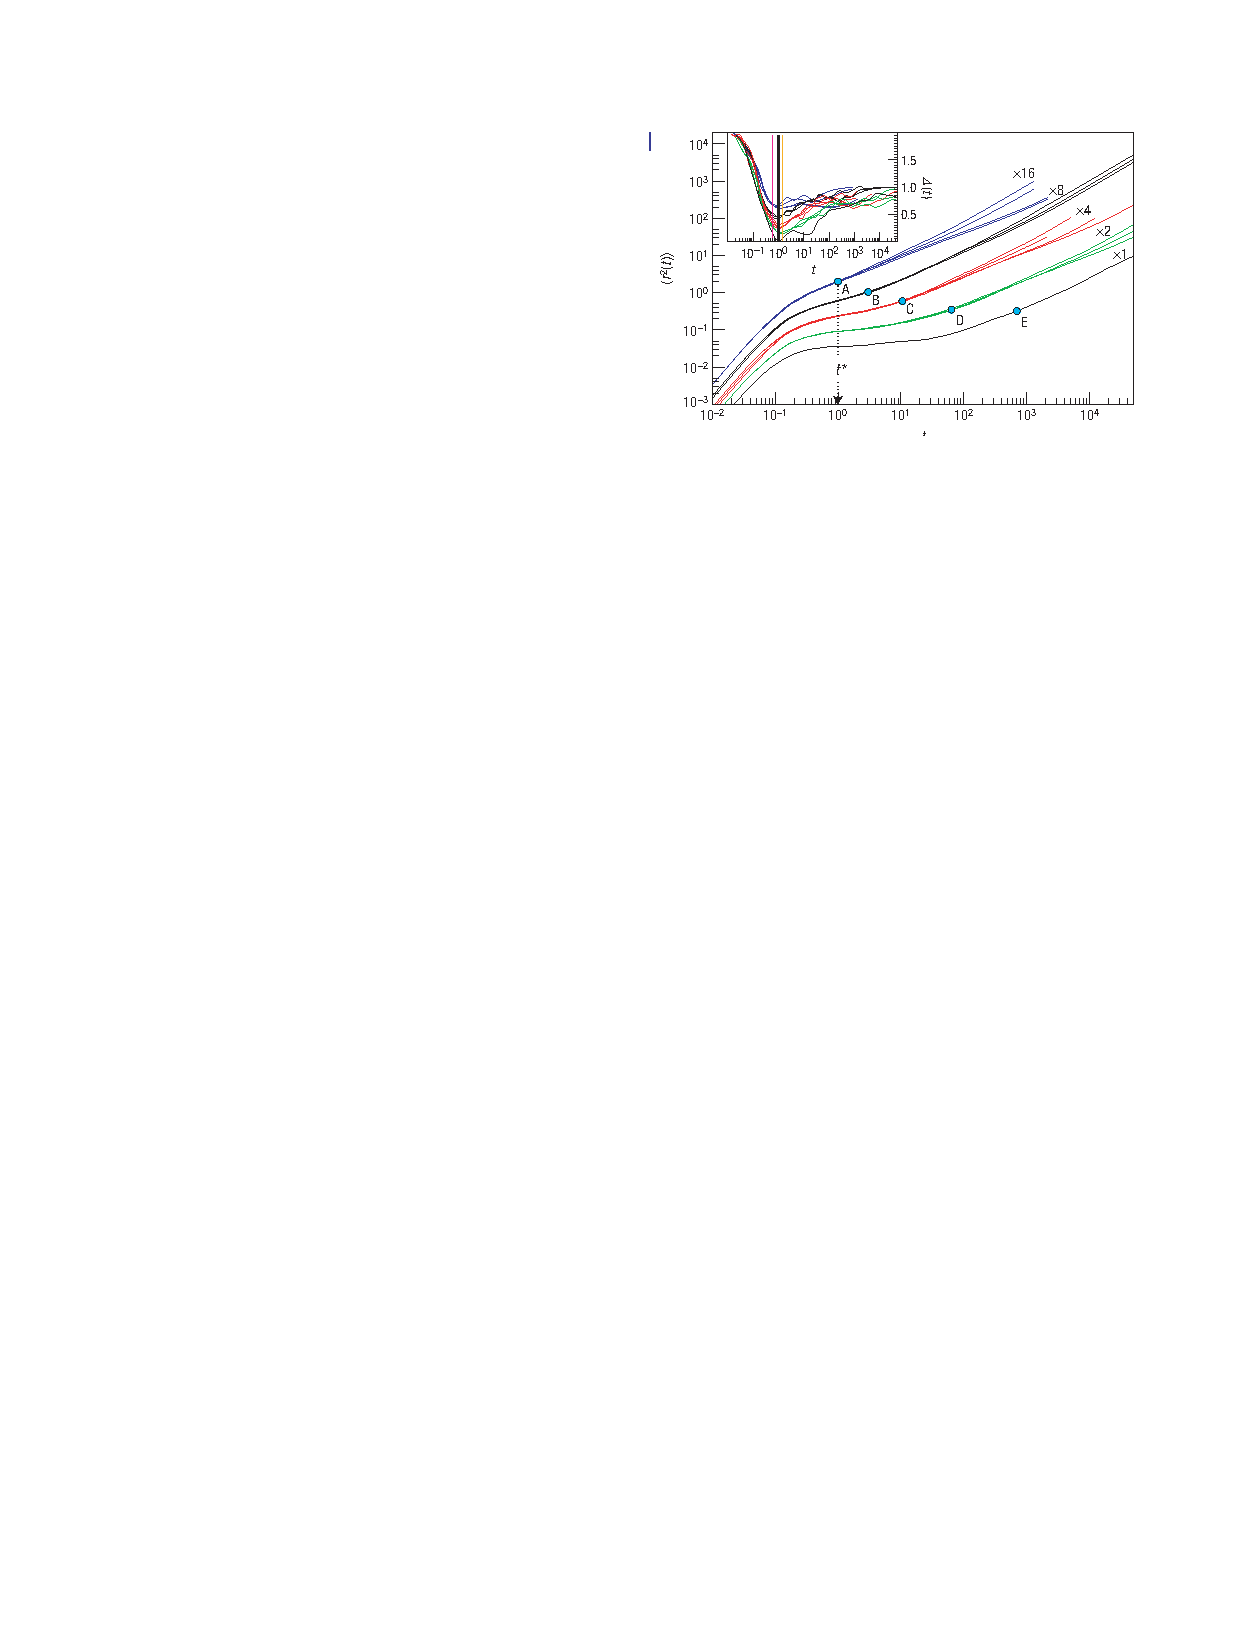
\includegraphics[width=\linewidth]{DW-ex}\\
            \onlinecite{larini:07}
        \end{column}
    \end{columns}
\end{frame}

\begin{frame}{Structural Rigidity}
    \centering
    \includegraphics[width=\textwidth]{{{DW.D}}}
\end{frame}

\section{Crystallisation}

\subsection{Crystal Structure}

\begin{frame}{Unit Cells}
    \begin{columns}
        \begin{column}{0.5\linewidth}
            \begin{itemize}
                \item The building blocks of crystals
                \item Can be used to tile all of space
            \end{itemize}
        \end{column}
        \begin{column}{0.5\linewidth}
            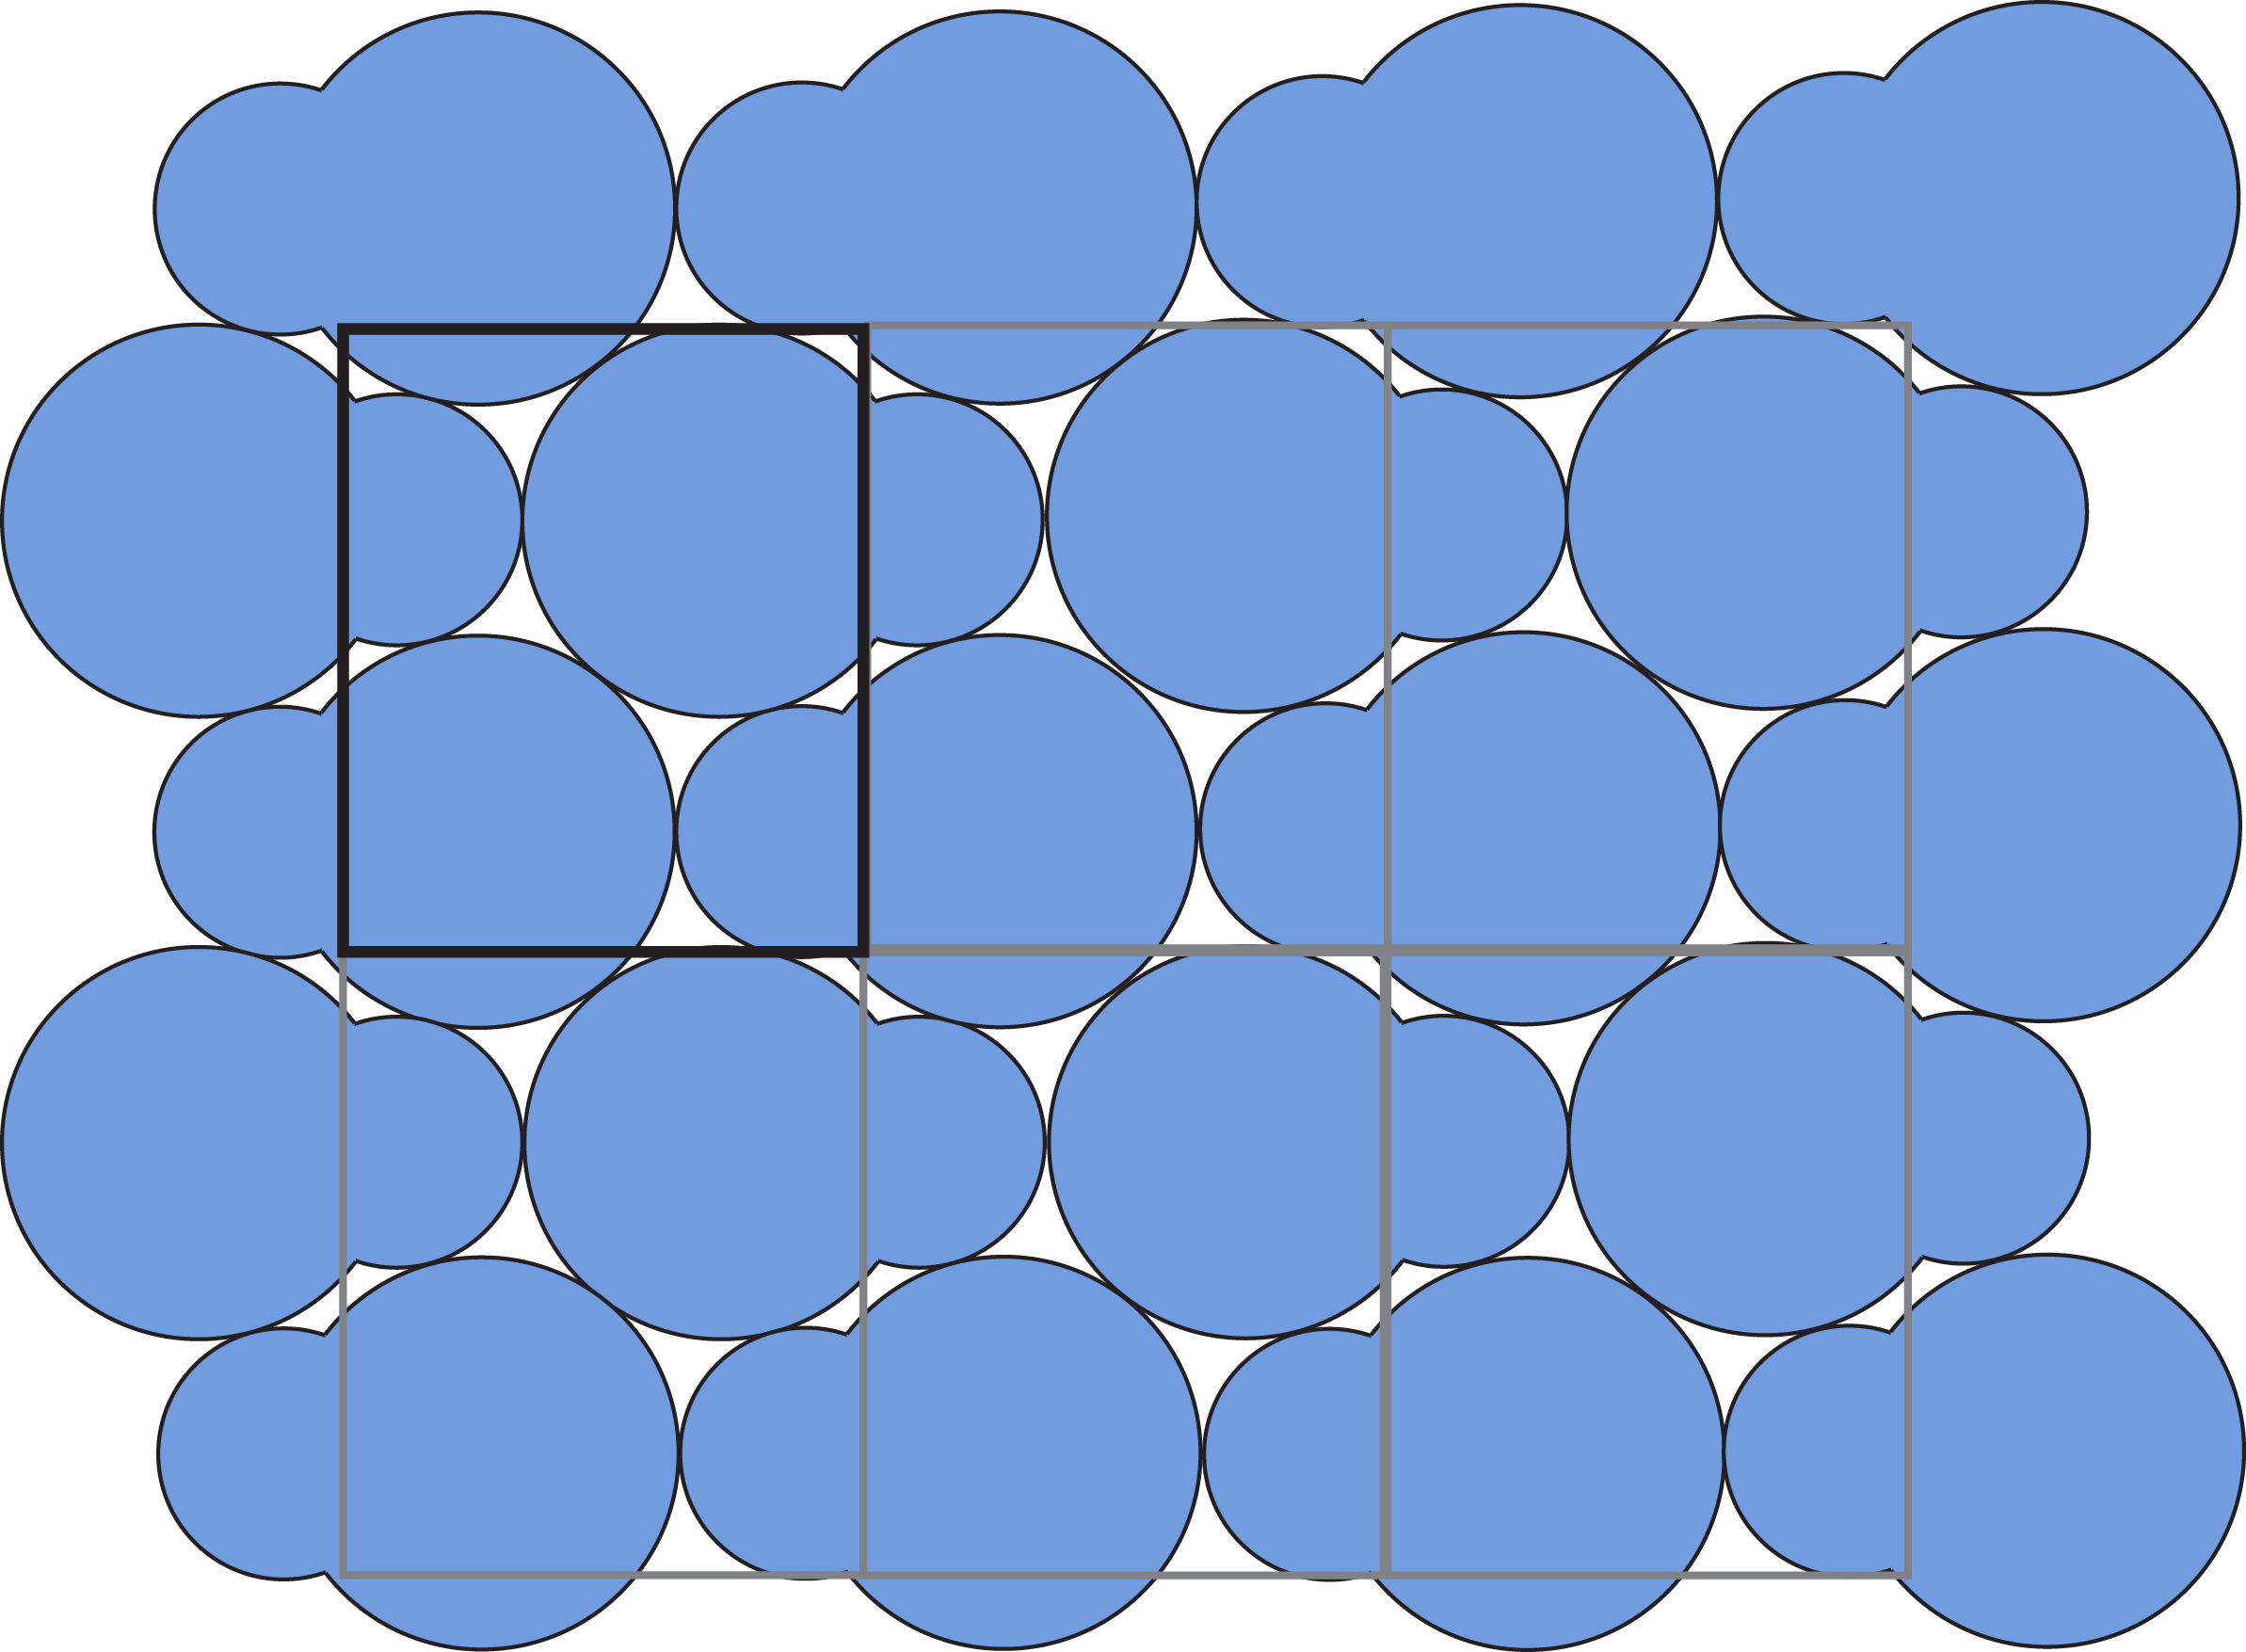
\includegraphics[width=\textwidth]{unit_cell}
        \end{column}
    \end{columns}
\end{frame}

\begin{frame}{Wallpaper Groups}
    \begin{columns}
        \begin{column}{0.5\linewidth}
            \begin{itemize}
                \item Give us the symmetry elements
                \item Minimal representation of the unit cell
            \end{itemize}
        \end{column}
        \begin{column}{0.5\linewidth}
            \centering
            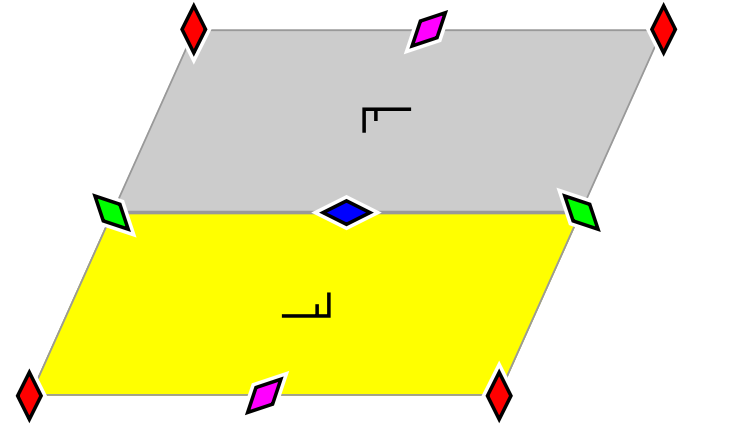
\includegraphics[width=0.8\textwidth]{p2}\\
            p2\\
            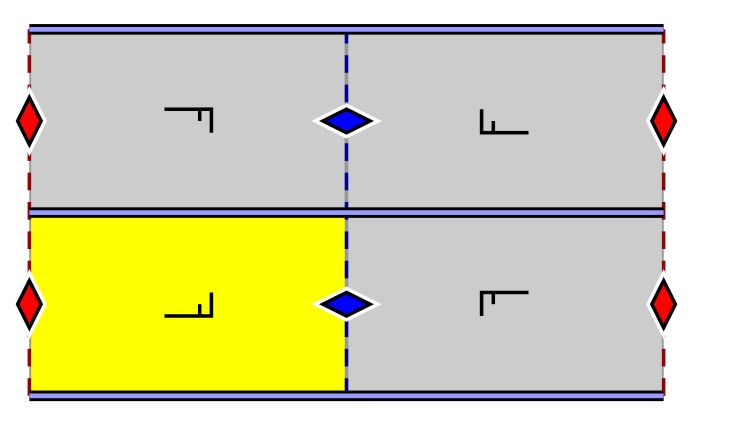
\includegraphics[width=0.8\textwidth]{p2mg}\\
            p2mg
        \end{column}
    \end{columns}
\end{frame}

\begin{frame}{Stable Crystals}
    \begin{columns}
        \begin{column}{0.5\linewidth}
            \centering
            \includegraphics[width=\linewidth]{{{Snowman-0.4-0.637556-1.00-p2mg-frame}}}
            \\\done p2mg
        \end{column}
        \begin{column}{0.5\linewidth}
            \centering
            \includegraphics[width=\linewidth]{{{Trimer-0.4-0.637556-1.00-120-p2-frame}}}
            \\\tri p2
        \end{column}
    \end{columns}
\end{frame}

\begin{frame}{Identifying the Crystal Phase}
    \begin{columns}
        \begin{column}{0.5\linewidth}
            \begin{itemize}
                \item Parallel and antiparallel alignment of molecules
                \item Use local orientations to describe order
                    \begin{align*}
                        O_\text{local} &= \frac{1}{N_\text{neigh}}\sum_{i=1}^{N_\text{neigh}} (\vect{\hat e} \cdot \vect{\hat e_i})^2
                    \end{align*}
            \end{itemize}
        \end{column}
        \begin{column}{0.5\linewidth}
            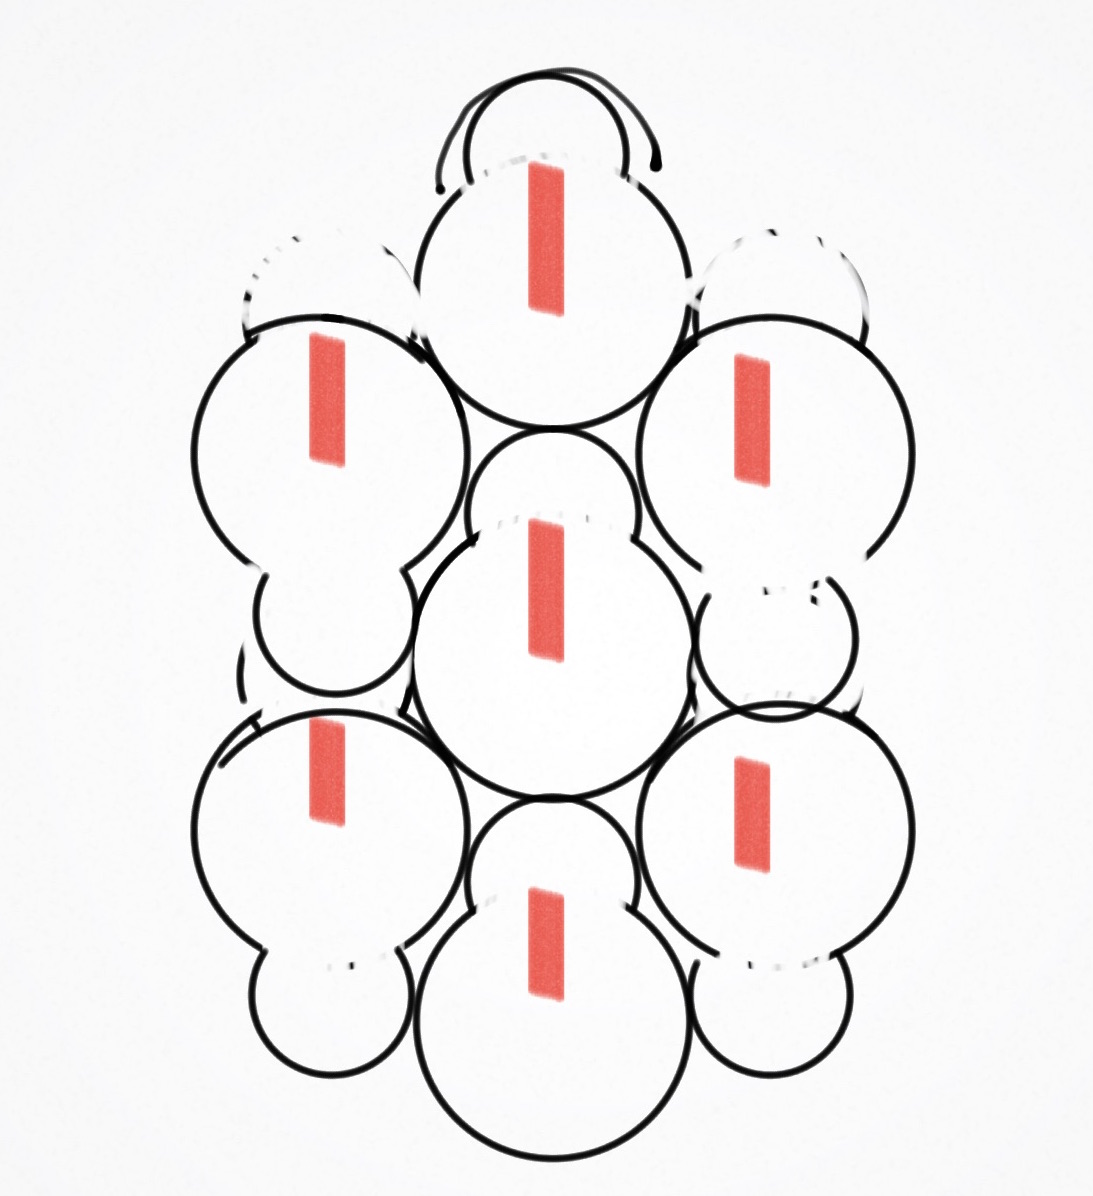
\includegraphics[width=\linewidth]{local-orientation}
        \end{column}
    \end{columns}
\end{frame}

\subsection{Crystal Dynamics}

\begin{frame}{Two Phase \tri}
    \noindent\makebox[\columnwidth]{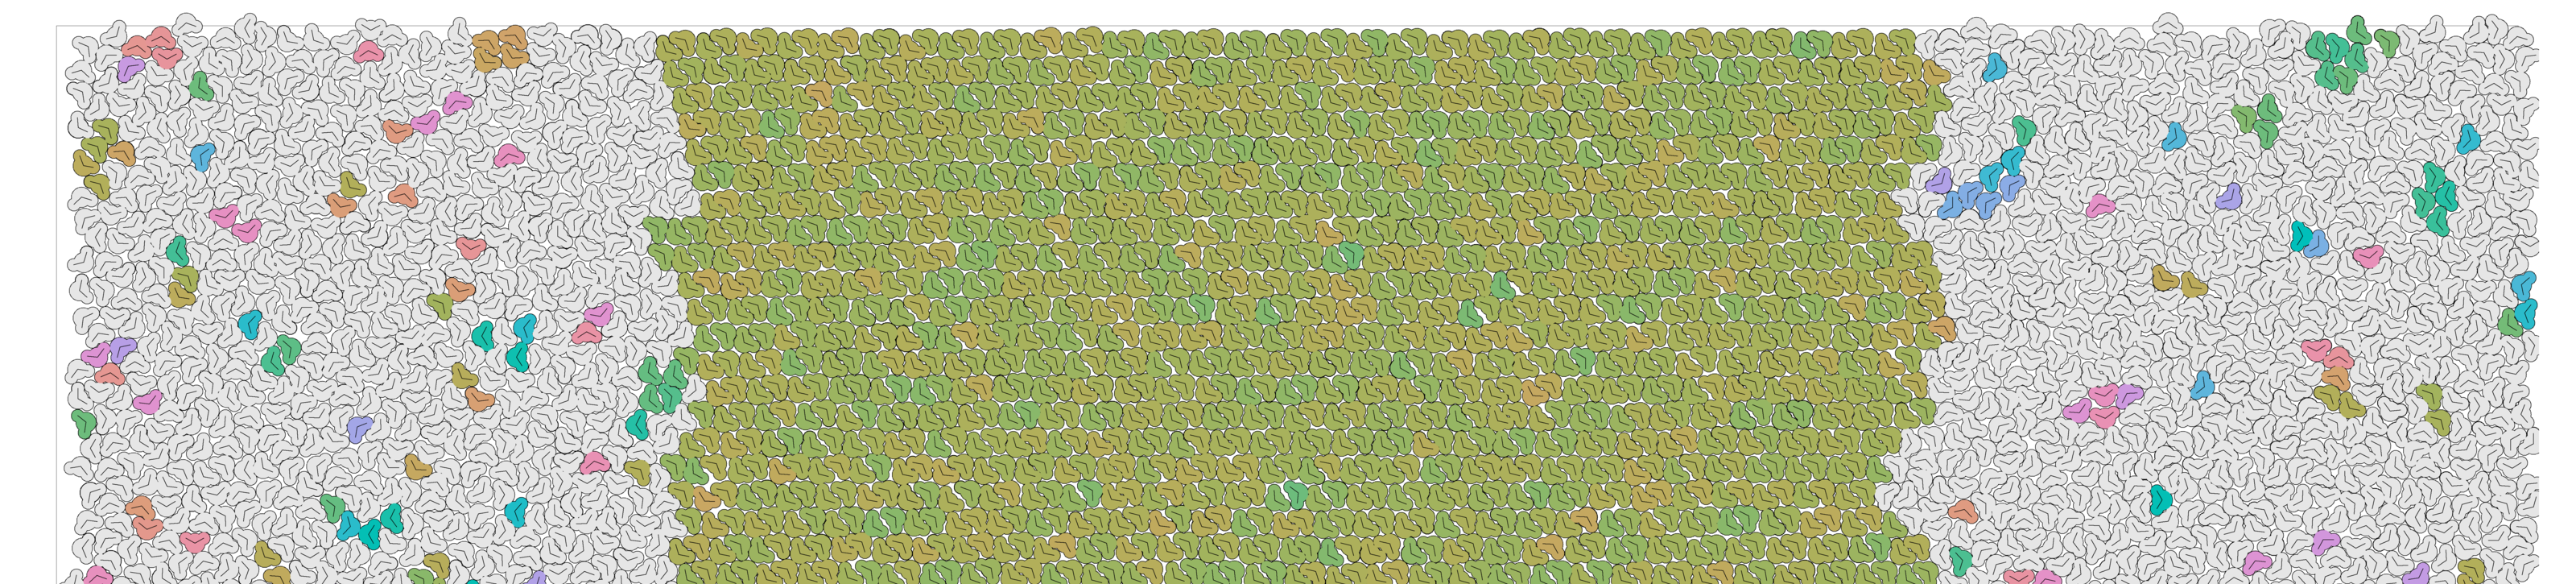
\includegraphics[width=\paperwidth]{tri-start}}
    \noindent\makebox[\columnwidth]{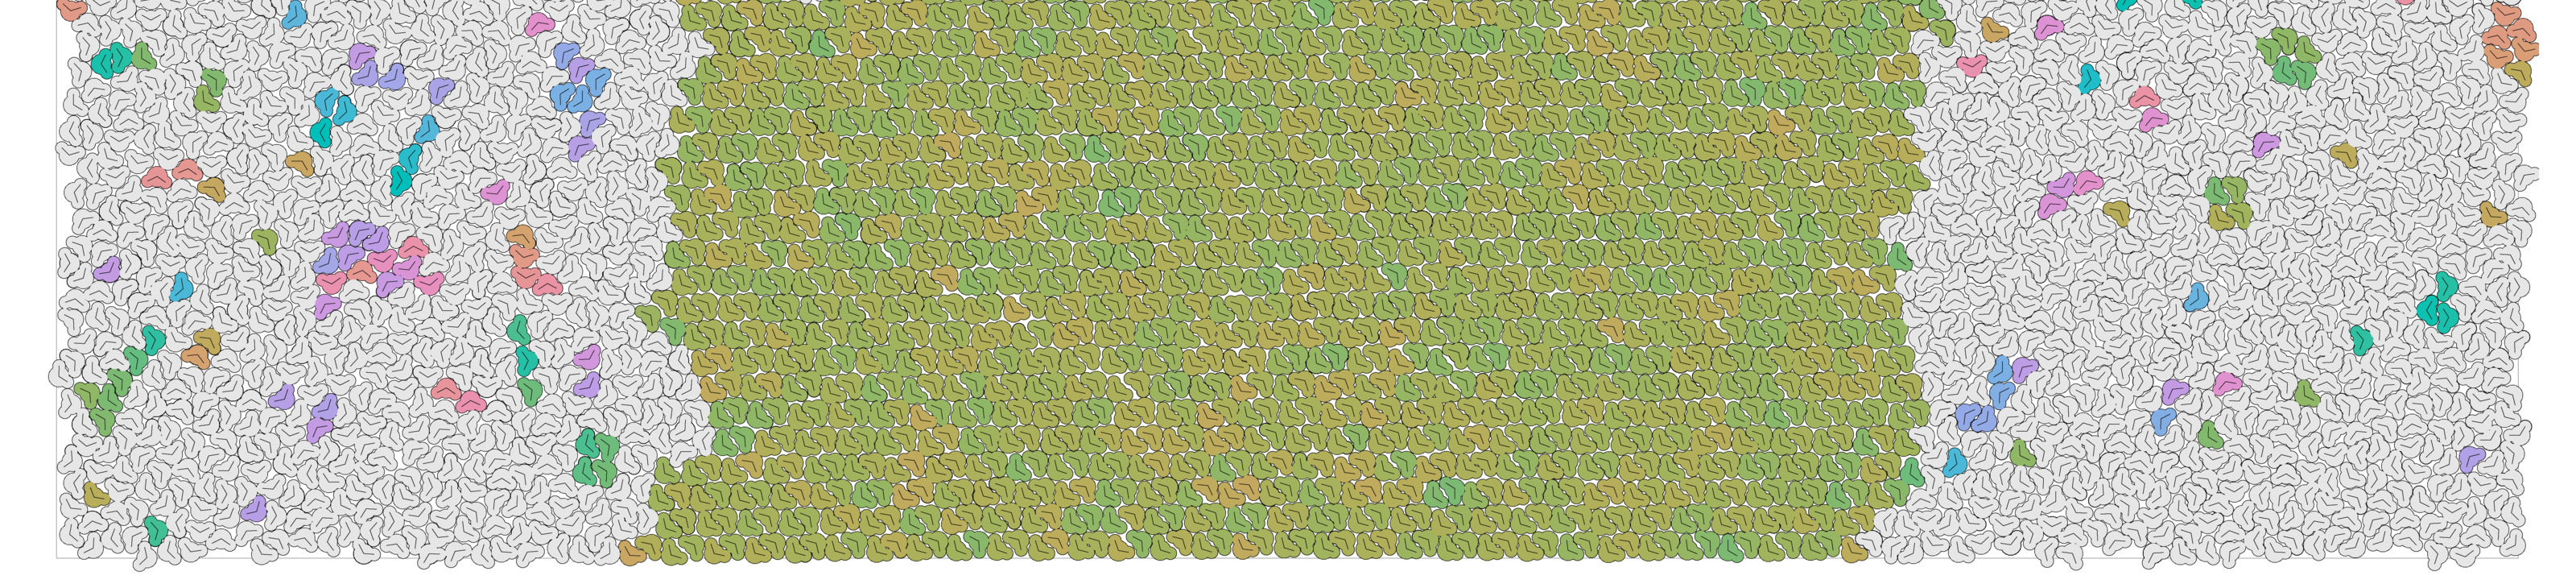
\includegraphics[width=\paperwidth]{tri-end}}
\end{frame}

\begin{frame}{Two Phase \done}
    \noindent\makebox[\columnwidth]{\includegraphics[width=\paperwidth]{done-start}}
    \noindent\makebox[\columnwidth]{\includegraphics[width=\paperwidth]{done-end}}
\end{frame}

\begin{frame}{Nucleation}
    \vspace{-3pt}
    \animategraphics[width=\linewidth]{12}{presentation/movie/}{0001}{0333}% replace with 0333
\end{frame}

\begin{frame}{Crystal Growth Rates}
    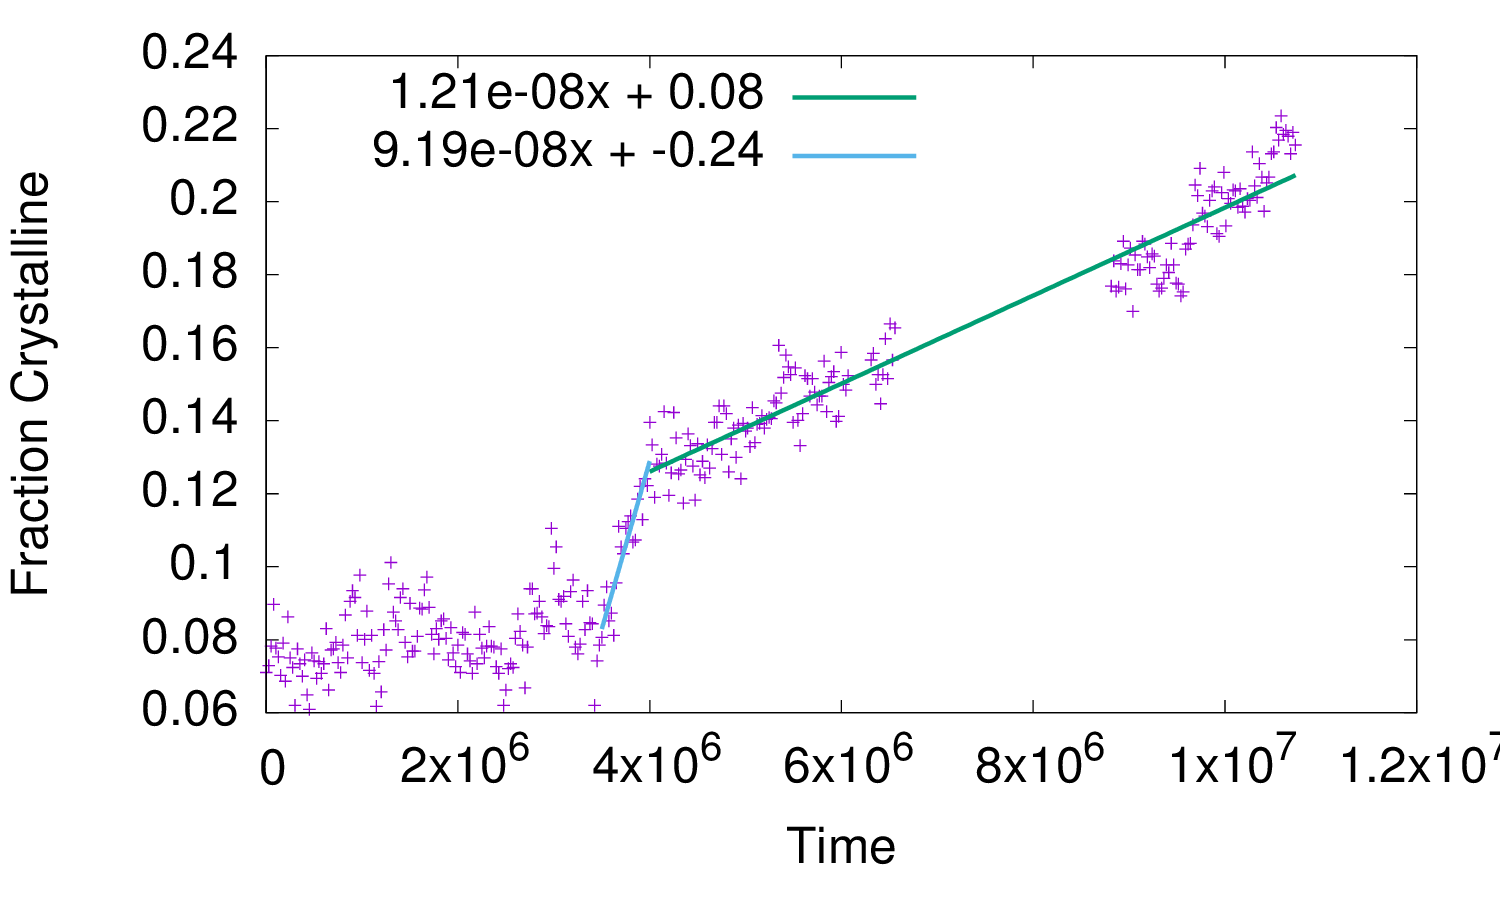
\includegraphics[width=\linewidth]{crys_growth}
\end{frame}

\section{Conclusion}

\begin{frame}{Conclusion}
    \begin{itemize}
        \item Small changes in molecular shape lead to order of magnitude differences in dynamics.
        \item Much of the differences in dynamics can be explained by the local structural rigidity.
        \item Molecular shape influences the crystal structure that can form.
        \item Crystallisation of these molecules occurs at temperatures where the dynamics are incredibly slow.
    \end{itemize}
\end{frame}

\begin{frame}{Questions}
    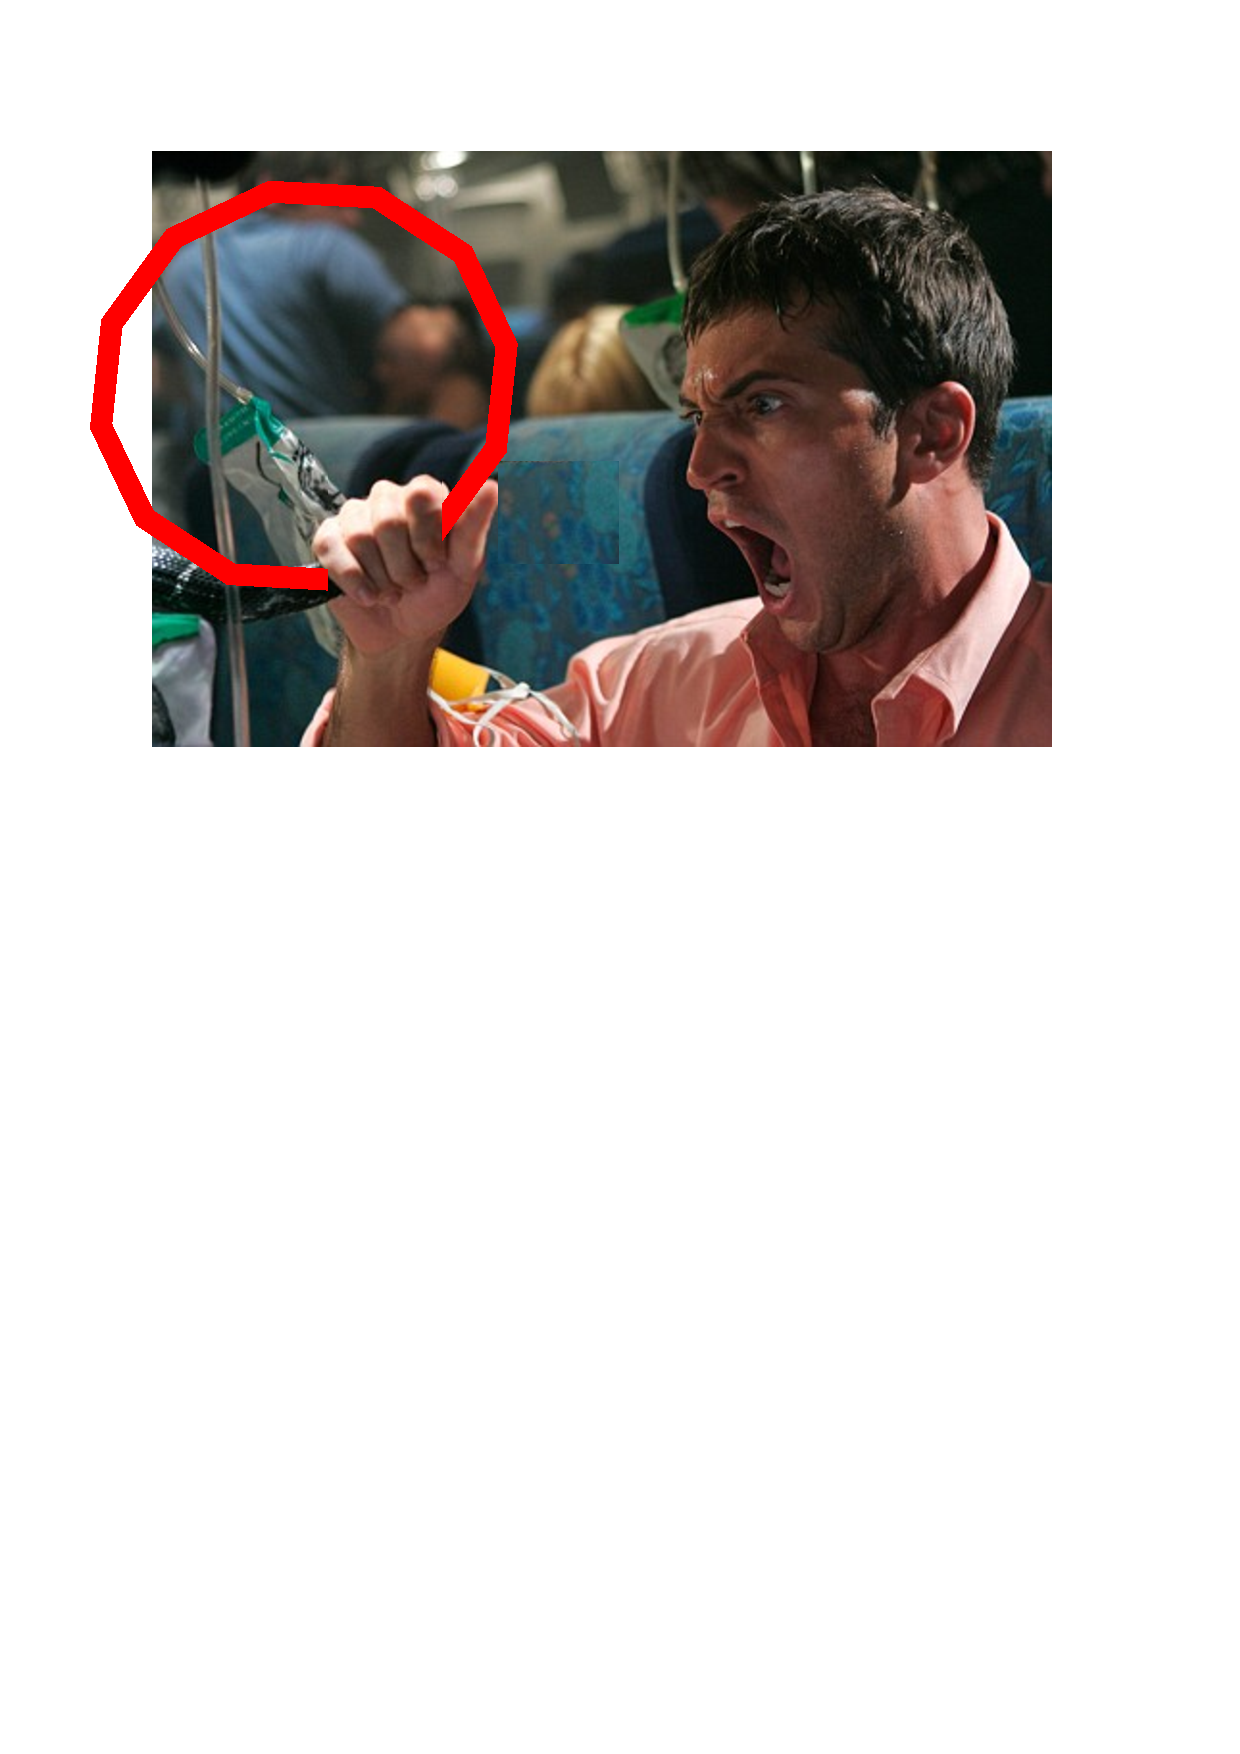
\includegraphics[width=\textwidth]{ahhh}
\end{frame}

\end{document}


